\documentclass[oneside,numbers,spanish]{ezthesis}
\usepackage[utf8]{inputenc}
\usepackage{tcolorbox}
\usepackage{listings}
\usepackage{graphicx}
\usepackage{pdfpages}
\usepackage{lscape}
\usepackage{xcolor}
\usepackage{todonotes}
\usepackage{lipsum}
\usepackage{bbding}
\usepackage{pifont}
\usepackage{wasysym}
\usepackage{fancyvrb}
\usepackage{amssymb}
\usepackage{natbib}
\usepackage{bm}
\usepackage{color}    
\usepackage{enumitem}
\usepackage{float}
\tcbuselibrary{skins,xparse}
\usepackage{varwidth}
\usepackage{lipsum}

\usepackage{hyperref}
\hypersetup{
    colorlinks,
    citecolor=black,
    filecolor=black,
    linkcolor=black,
    urlcolor=black
}


\definecolor{blue}{rgb}{0.0, 0.22, 0.66}
\definecolor{YellowGreen}{rgb}{0.31, 0.49, 0.16}
\definecolor{ForestGreen}{rgb}{0.31, 0.49, 0.16}
\definecolor{RoyalBlue}{rgb}{0.58,0,0.82}
\definecolor{mygray}{gray}{0.96}
\definecolor{backcolour}{rgb}{0.95,0.95,0.92}
%\definecolor{aurometalsaurus}{rgb}{0.43, 0.5, 0.5}
 \definecolor{aurometalsaurus}{rgb}{0.52, 0.52, 0.51}
\usepackage{titlesec}
\setlist[itemize]{noitemsep, topsep=0pt}

\setlength{\parskip}{4pt}
 
\makeatletter
\def\myaddcontentsline#1#2#3{%
  \addtocontents{#1}{\protect\contentsline{#2}{#3}{see \thesection\ at p. \thepage}{}}}
\renewcommand{\@todonotes@addElementToListOfTodos}{%
    \if@todonotes@colorinlistoftodos%
        \myaddcontentsline{tdo}{todo}{{%
            \colorbox{\@todonotes@currentbackgroundcolor}%
                {\textcolor{\@todonotes@currentbackgroundcolor}{o}}%
            \ \@todonotes@caption}}%
    \else%
        \myaddcontentsline{tdo}{todo}{{\@todonotes@caption}}%
    \fi}%
\newcommand*\mylistoftodos{%
  \begingroup
       \setbox\@tempboxa\hbox{see 9.9 at p. 99}%
       \renewcommand*\@tocrmarg{\the\wd\@tempboxa}%
       \renewcommand*\@pnumwidth{\the\wd\@tempboxa}%
       \listoftodos%
  \endgroup
}
\makeatother


\lstset{
basicstyle=\footnotesize,
keywordstyle=\bfseries,
showstringspaces=false,
backgroundcolor=\color{backcolour}, 
numbersep=4pt, 
columns = fullflexible,
tabsize=2,                      % sets default tabsize to 2 spaces
captionpos=b,                   % sets the caption-position to bottom
breaklines=true,                % sets automatic line breaking
mathescape = true,
breakatwhitespace=false,        % sets if automatic breaks should only happen at whitespace
language=R,
linewidth=0.95\columnwidth,
xleftmargin=0.5cm,
%frame = single,  
framexleftmargin=15pt,
keywordstyle=\color{blue},      % keyword style
commentstyle=\color{YellowGreen}   % comment style
%stringstyle=\color{ForestGreen}      % string literal style
}


 



%% # Opciones disponibles para el documento #
%%
%% Las opciones con un (*) son las opciones predeterminadas.
%%
%% Modo de compilar:
%%   draft            - borrador con marcas de fecha y sin im'agenes
%%   draftmarks       - borrador con marcas de fecha y con im'agenes
%%   final (*)        - version final de la tesis
%%
%% Tama'no de papel:
%%   letterpaper (*)  - tama'no carta (Am'erica)
%%   a4paper          - tama'no A4    (Europa)
%%
%% Formato de impresi'on:
%%   oneside          - hojas impresas por un solo lado
%%   twoside (*)      - hijas impresas por ambos lados
%%
%% Tama'no de letra:
%%   10pt, 11pt, o 12pt (*)
%%
%% Espaciado entre renglones:
%%   singlespace      - espacio sencillo
%%   onehalfspace (*) - espacio de 1.5
%%   doublespace      - a doble espacio
%%
%% Formato de las referencias bibliogr'aficas:
%%   numbers          - numeradas, p.e. [1]
%%   authoryear (*)   - por autor y a'no, p.e. (Newton, 1997)
%%
%% Opciones adicionales:
%%   spanish         - tesis escrita en espa'nol
%%
%% Desactivar opciones especiales:
%%   nobibtoc   - no incluir la bibiolgraf'ia en el 'Indice general
%%   nofancyhdr - no incluir "fancyhdr" para producir los encabezados
%%   nocolors   - no incluir "xcolor" para producir ligas con colores
%%   nographicx - no incluir "graphicx" para insertar gr'aficos
%%   nonatbib   - no incluir "natbib" para administrar la bibliograf'ia

%% Paquetes adicionales requeridos se pueden agregar tambi'en aqu'i.
%% Por ejemplo:
%\usepackage{subfig}
%\usepackage{multirow}

%% # Datos del documento #
%% Nota que los acentos se deben escribir: \'a, \'e, \'i, etc.
%% La letra n con tilde es: \~n.

\author{JULIA ANGELINI}
\title{Paquete de R y aplicación Web para el análisis de datos provenientes de ensayos multiambientales}
\degree{TRABAJO FINAL PARA OPTAR AL TITULO DE ESPECIALISTA EN BIOINFORMÁTICA}
\supervisor{DIRECTOR: Gerardo Cervigni \\
			CO-DIRECTOR: Marcos Prunello}
\institution{UNIVERSIDAD NACIONAL DE ROSARIO}
\faculty{FACULTAD DE CIENCIAS AGRARIAS}
\submitdate{AÑO: 2020}
%% # M'argenes del documento #
%% 
%% Quitar el comentario en la siguiente linea para austar los m'argenes del
%% documento. Leer la documentaci'on de "geometry" para m'as informaci'on.

\geometry{top=30mm,bottom=30mm,inner=30mm,outer=20mm}

 
%% El siguiente comando agrega ligas activas en el documento para las
%% referencias cruzadas y citas bibliogr'aficas. Tiene que ser *la 'ultima*
%% instrucci'on antes de \begin{document}.
%\hyperlinking
\begin{document}

%% En esta secci'on se describe la estructura del documento de la tesis.
%% Consulta los reglamentos de tu universidad para determinar el orden
%% y la cantidad de secciones que debes de incluir.

%% # Portada de la tesis #
%% Mirar el archivo "titlepage.tex" para los detalles.
\begin{titlepage}
  \TitleBlock{
  \centering 
\includegraphics[height=3cm, keepaspectratio=true]{./Graficos/UNR.png}
  
  \vspace*{0.15cm}
  \normalsize \scshape \textbf{\insertfaculty} \\
  \vspace*{0.15cm}
  \textbf{\insertinstitution}
	}
  \TitleBlock[\vspace*{1.5cm}]{\large\scshape \textbf{\inserttitle}}
  \vspace*{0.55cm}

  \TitleBlock[\vspace*{1.5cm}]{\normalsize \scshape \textbf{\insertauthor}}
  \TitleBlock[\vspace*{0.75cm}]{\normalsize \scshape \textbf{\insertdegree} \\
  \rule{5cm}{0.2mm}}
  \TitleBlock[\vspace*{1.5cm}]{\normalsize \scshape 
  \textbf{\insertsupervisor}}
  \TitleBlock[\vspace*{1.5cm}]{\textbf{\insertsubmitdate}}
\end{titlepage}


%% # Prefacios #
%% Por cada prefacio (p.e. agradecimientos, resumen, etc.) crear
%% un nuevo archivo e incluirlo aqu'i.
%% Para m'as detalles y un ejemplo mirar el archivo "gracias.tex".
%% Las secciones del "prefacio" inician con el comando \prefacesection{T'itulo}
%% Este tipo de secciones *no* van numeradas, pero s'i aparecen en el 'indice.
%%
%% Si quieres agregar una secci'on que no vaya n'umerada y que *tampoco*
%% aparesca en el 'indice, usa entonces el comando \chapter*{T'itulo}
%%
%% Recuerda que aqu'i ya puedes escribir acentos como: 'a, 'e, 'i, etc.
%% La letra n con tilde es: 'n.

%\thispagestyle{empty}
\begin{center}
\textbf{\Large{Paquete de R y aplicación web Shiny para el análisis de datos provenientes de ensayos multiambientales}}
\end{center}

\vspace{1.5cm}

\begin{center}
Julia Angelini

\vspace{0.5cm}
Licenciada en Estadística – Universidad Nacional de Rosario
\end{center}
\vspace{1.5cm}
Este Trabajo Final es presentado como parte de los requisitos para optar al grado académico de Especialista en \textbf{Bioinformática}, de la Universidad Nacional de Rosario y no ha sido previamente presentada para la obtención de otro título en ésta u otra Universidad. El mismo contiene los resultados obtenidos en investigaciones llevadas a cabo en \textbf{el Centro de Estudios Fotosintéticos y Bioquímicos (CEFOBI)}, durante el período comprendido entre \textbf{los años 2017 y 2021}, bajo la dirección del \textbf{Dr. Gerardo Cervigni} y la co-dirección del \textbf{Mgs. Marcos Prunello}.  

\vspace{1.25cm}
Nombre y firma del autor\\
\vspace{0.05cm}
\hspace{0.95cm}Lic. Julia Angelini

\vspace{1.25cm}
Nombre y firma del Director\\
\vspace{0.05cm}
\hspace{0.95cm}Dr. Gerardo Cervigni
 
\vspace{1.25cm}
Nombre y firma del Co - Director\\
\vspace{0.05cm}
\hspace{1.3cm}Mgs. Marcos Prunello
\vspace{1.85cm}

\rightline{Defendida: \rule{3cm}{0.4pt} de 20\rule{1cm}{0.4pt}.}


%% Por si alguien tiene curiosidad, este "simp'atico" agradecimiento est'a
%% tomado de la "Tesis de Lydia Chalmers" basada en el universo del programa
%% de televisi'on Buffy, la Cazadora de Vampiros.
%% http://www.buffy-cazavampiros.com/Spiketesis/tesis.inicio.htm


\pagestyle{plain}
\pagenumbering{roman}
%% Las secciones del "prefacio" inician con el comando \prefacesection{T'itulo}
%% Este tipo de secciones *no* van numeradas, pero s'i aparecen en el 'indice.
%%
%% Si quieres agregar una secci'on que no vaya n'umerada y que *tampoco*
%% aparesca en el 'indice, usa entonces el comando \chapter*{T'itulo}
%%
%% Recuerda que aqu'i ya puedes escribir acentos como: 'a, 'e, 'i, etc.
%% La letra n con tilde es: 'n.

\chapter*{Agradecimientos}
\begin{spacing}{1}

\emph{En este trabajo final, directa o indirectamente, participaron muchas personas a las que les quiero agradecer.}

\emph{En primer lugar al Dr. Gerardo Cervigni por haberme propuesto realizar la Especialización Bioinformática, compartir su conocimiento y experiencia a lo largo de todo el proceso, contagiando su pasión, entusiasmo y energía. }

\emph{Al Mgs. Marcos Prunello por acompañarme en el desarrollo del trabajo final, por su dedicación, sus consejos y su ejemplo que me incentiva a superarme como profesional. Sin su confianza, apoyo y atención, este trabajo no hubiera sido posible. No sólo me enriquecí en lo académico sino también con la amistad que pudimos forjar. }

\emph{Al Centro Computacional del Centro Científico Teconológico de Rosario, miembro del Sistema Nacional de Computación de Alto Rendimiento, por la predisposición, asesoramiento e instalación de los recursos adicionales necesarios para este trabajo. }

\emph{Al Dr. Sergio Arciniegas Alarcón por su predisposición en la inclusión de los avances metodológicos realizados por su equipo de investigación en este trabajo.}

\emph{A mis compañeros de la Especialización, por las largas horas de cursos, mates y almuerzos. En especial, a Jor y Lu, por el aliento en todo momento, por compartir excelentes momentos y porque gracias a la ayuda de ambas he podido entender cosas que no habría podido sola.}

\emph{A los docentes de la Especialización en Bioinformática por su dedicación y paciencia para enseñarle a alumnos provenientes de las más diversas áreas esta hermosa combinación entre Biología, Informática y Estadística.}

\emph{A mis padres por el amor y apoyo incondicional y por el esfuerzo  de  dedicar  sus  vidas  a  brindarnos  a mi hermano y a mí la  posibilidad  de construir nuestros futuros. A mi hermano, por su cariño, apoyo, acompañamiento y sentido del humor. A Otto, por su incomparable mezcla de amor y comprensión, por darme fuerzas en los momentos de debilidad y por alentarme a seguir a pesar de todo. A Segundo, Mia y Kalita, por su hermosa compañía día a día.}

\emph{Por último, pero no menos importante, a Gaby y Euge mis compañeras de CEFOBI, por acompañarme en las partes más empedradas del camino, por compartir las risas y las  lágrimas, por su amistad y consejos. No hubiese alcanzado mucho de mis logros sin su ayuda, compañía y aliento en todo momento.}
\end{spacing}



%% Por si alguien tiene curiosidad, este "simp'atico" agradecimiento est'a
%% tomado de la "Tesis de Lydia Chalmers" basada en el universo del programa
%% de televisi'on Buffy, la Cazadora de Vampiros.
%% http://www.buffy-cazavampiros.com/Spiketesis/tesis.inicio.htm

%% Los cap'itulos inician con \chapter{T'itulo}, estos aparecen numerados y
%% se incluyen en el 'indice general.
%%
%% Recuerda que aqu'i ya puedes escribir acentos como: 'a, 'e, 'i, etc.
%% La letra n con tilde es: 'n.


\chapter*{Abreviaturas}
%\thispagestyle{empty}
\begin{spacing}{1}
\begin{description}
\item{\textbf{ACP}}: análisis de componentes principales.

\item{\textbf{AEC}}: coordenada ambiental promedio (siglas en inglés de \emph{Average environment coordination}).

\item{\textbf{ANOVA}}: análisis de la variancia (siglas en inglés de \emph{analysis of variance}).

\item{\textbf{AMMI}}: modelo de efectos principales aditivos e interacción multiplicativa (siglas en inglés de \emph{Additive Main effects and Multiplicative Interaction}).

\item{\textbf{CCT}}: Centro Científico Teconológico.

\item{\textbf{COI}}: interacción con cambio de rango (siglas en inglés de \emph{crossover interaction}).

\item{\textbf{CONICET}}: Consejo Nacional de Investigaciones Científicas y Técnicas.

\item{\textbf{CRAN}}: \emph{Comprehensive R Archive Network}.

\item{\textbf{DVS}}: descomposición de valores singulares.

\item{\textbf{EM}}: maximización de la esperanza (siglas en inglés de \emph{Expectation Maximization}).

\item{\textbf{EMA}}: ensayos multiambientales.

\item{\textbf{G}}: efecto genotípico.

\item{\textbf{GE}}: genotipo-ambiente (siglas en inglés de \emph{Genotype-Environment}).

\item{\textbf{GGE}}: genotipo más genotipo-ambiente (siglas en inglés de \emph{Genotype plus Genotype-Environment}).

\item{\textbf{IGA}}: interacción genotipo-ambiente.

\item{\textbf{NCOI}}: interacción sin cambio de rango (siglas en inglés de \emph{no crossover interaction}).

\item{\textbf{SREG}}: modelo de regresión por sitio (siglas en inglés de \emph{Site Regression model}).

\item{\textbf{SVP}}: partición de los valores singulares (siglas en inglés de \emph{Singular Value Partition}).

\item{\textbf{ui}}: interfaz del usuario (siglas en inglés de \emph{user interface}).


\end{description}
\end{spacing}
%% Las secciones del "prefacio" inician con el comando \prefacesection{T'itulo}
%% Este tipo de secciones *no* van numeradas, pero s'i aparecen en el 'indice.
%%
%% Si quieres agregar una secci'on que no vaya n'umerada y que *tampoco*
%% aparesca en el 'indice, usa entonces el comando \chapter*{T'itulo}
%%
%% Recuerda que aqu'i ya puedes escribir acentos como: 'a, 'e, 'i, etc.
%% La letra n con tilde es: 'n.

\chapter*{Resumen}

%\thispagestyle{empty}
Las variedades mejoradas de cultivos vegetales son el resultado del trabajo de desarrollo genético llevado a cabo en los programas de fitomejoramiento, los cuales se extienden a lo largo de varios años y requieren cuantiosas inversiones. En etapas avanzadas, los ensayos multiambientales (EMA), que comprenden experimentos en múltiples ambientes, son herramientas fundamentales para incrementar la productividad y rentabilidad de los cultivos. La vigencia comercial de las variedades puede extenderse durante varias décadas, por lo que su elección es crítica para que el productor evite pérdidas económicas por malas campañas y el suministro al mercado sea constante. Consecuentemente, un análisis adecuado de la información de los EMA es indispensable para que el programa de mejoramiento de cultivos sea efiecaz. Actualmente, R es uno de los lenguajes de programación más utilizados para el análisis de datos debido a su distribución como software libre y a la gran variedad de herramientas que ofrece. Sin embargo, los mejoradores que no están familiarizados con la programación tienden a utilizar otros tipos de programas que responden a instrucciones por menú en lugar de escribir lineas de código, a pesar de los costos económicos derivados del pago de sus licencias. Mientras que, aquellos que sí tienen afinidad con el uso de código para el análisis de datos se enfrentan con dificultades a la hora de identificar las herramientas aporpiadas entre el gran número de instrumentos disponibles. Por lo tanto, en este trabajo se presenta el desarrollo de dos herramientas informáticas para asistir en el análisis de datos provenientes de EMA. Por un lado, se creó un nuevo paquete de R que propone funciones nuevas y al mismo tiempo reúne todas aquellas de mayor utilidad, de modo que aquellos usuarios que posean un manejo del lenguaje puedan simplificar su tarea. Por otro lado, se confeccionó una interfaz gráfica de usuario mediante una aplicación web Shiny que permite realizar los principales análisis implementados en el paquete sin necesidad de programar y se encuentra publicada en internet en el servidor de CONICET para su libre acceso.

\textbf{Palabras Clave: ensayos multiambientales, estadística, interfaz gráfica, programación}

%% Por si alguien tiene curiosidad, este "simp'atico" agradecimiento est'a
%% tomado de la "Tesis de Lydia Chalmers" basada en el universo del programa
%% de televisi'on Buffy, la Cazadora de Vampiros.
%% http://www.buffy-cazavampiros.com/Spiketesis/tesis.inicio.htm

\include{abstract}


%% # 'Indices y listas de contenido #
%% Quitar los comentarios en las lineas siguientes para obtener listas de
%% figuras y cuadros/tablas.
\setcounter{secnumdepth}{4}
\setcounter{tocdepth}{4}

\addtocontents{toc}{\hspace{-7.5mm} \textbf{Capítulos}}
\addtocontents{toc}{\hfill \textbf{Página} \par}
\addtocontents{toc}{\vspace{-2mm} \hspace{-7.5mm} \hrule \par}
\tableofcontents
\cleardoublepage

\listoffigures
\cleardoublepage

%%\renewcommand{\listtablename}{Índice de tablas}
%%\renewcommand{\tablename}{Tabla}
%%\listoftables
%%\cleardoublepage

%% # Cap'itulos #
%% Por cada cap'itulo hay que crear un nuevo archivo e incluirlo aqu'i.
%% Mirar el archivo "intro.tex" para un ejemplo y recomendaciones para
%% escribir.

%%Lista de comentarios
%%\pagestyle{plain}
%%\mylistoftodos
%%\cleardoublepage

\pagestyle{plain}
\pagenumbering{arabic}

%% Los cap'itulos inician con \chapter{T'itulo}, estos aparecen numerados y
%% se incluyen en el 'indice general.
%%
%% Recuerda que aqu'i ya puedes escribir acentos como: 'a, 'e, 'i, etc.
%% La letra n con tilde es: 'n.


\chapter{Introducción}

A lo largo de la historia de la agricultura, el hombre ha desarrollado el mejoramiento vegetal (o fitomejoramiento) en forma sistemática y lo ha convertido en un instrumento esencial para la mejora de la producción agrícola en términos de cantidad, calidad y diversidad.  

La humanidad depende, directa o indirectamente, de las plantas. Para la alimentación, ya que todos sus alimentos son vegetales o se derivan de éstos por ejemplo: carne, huevos y productos lácteos. De las plantas se deriva también la mayoría de las fibras textiles, fármacos, combustibles, lubricantes y materiales de construcción.

El fitomejoramiento, en un sentido amplio, es el arte y la ciencia de alterar o modificar la herencia de las plantas para obtener cultivares (variedades o híbridos) mejorados genéticamente, adaptados a condiciones específicas, de mayores rendimientos económicos y de mejor calidad que las variedades nativas o criollas \citep{Allard67}. En otras palabras, el fitomejoramiento busca crear plantas cuyo patrimonio hereditario esté de acuerdo con las condiciones, necesidades y recursos de los productores rurales, de la industria y de los consumidores, o sea de todos aquellos que producen, transforman y consumen productos vegetales. 

Las variedades mejoradas son el resultado del trabajo de desarrollo genético llevado a cabo en los programas de fitomejoramiento, los cuales se extienden a lo largo de varios años y requieren cuantiosas inversiones. La vigencia comercial de las variedades puede extenderse varias décadas, por lo que su elección es crítica para que el productor evite pérdidas económicas por malas campañas y el suministro al mercado sea constante. 

Generalmente, en etapas tempranas de estos programas existen un gran número de genotipos experimentales con pocos antecedentes de evaluación; mientras que en etapas posteriores  se trabaja con pocos genotipos altamente selectos. 

La utilización adecuada de procedimientos de análisis de datos agronómicos y ambientales es una condición inherente al desarrollo actual y futuro de investigaciones orientadas a mejorar los cultivos en forma económica y ambientalmente sustentable. En etapas avanzadas de los programas de mejoramiento, los ensayos multiambientales (EMA) que comprenden experimentos en múltiples ambientes son herramientas fundamentales para incrementar la productividad y rentabilidad de los cultivos. Estos son frecuentes en investigaciones agricolas de comparación de rendimiento, ya que constituyen una de las principales estrategias de identificación de genotipos vegetales superiores y de ambientes en los cuales estos se expresan de manera diferencial.

Debido a que las regiones de producción de los principales cultivos cubren áreas ecológicas muy extensas, se observan variaciones en las condiciones climáticas y de suelo. Por lo tanto, la aparición de la interacción genotipo ambiente (IGA) es inevitable, provocando respuestas altamente variables en los diferentes ambientes (Crossa et al., 1990; Cruz Medina, 1992; Kang y Magari, 1996). La IGA es considerada casi unánimemente por los fitomejoradores como el principal factor que limita la respuesta a la selección y, en general, la eficiencia de los programas de mejoramiento. 

Los investigadores agrícolas han sido conscientes de las diversas implicaciones de IGA en los programas de mejoramiento (Mooers, 1921; Yates y Cochran, 1938). Por ejemplo, la IGA tiene un impacto negativo en la heredabilidad, cuanto menor sea la heredabilidad de un caracter, mayor será la dificultad para mejorar ese caracter mediante la selección.
Por lo tanto, información sobre la estructura y la naturaleza de la IGA es particularmente útil para los mejoradores porque puede ayudar a determinar si necesitan desarrollar cultivares para todos los ambientes de interés o si deberían desarrollar cultivares específicos para ambientes específicos (Bridges, 1989). Gauch y Zobel (1996) explicaron la importancia de IGA como: “Si no hubiera interacción, una sola variedad de trigo (\emph{Triticum aestivum} L.) o maíz (\emph{Zea mays} L.) o cualquier otro cultivo rendiria al máximo en todo el mundo, y además la prueba de variedades deberia realizarse en un sólo lugar para proporcionar resultados universales. No habría ruido, los resultados experimentales serían exactos, identificando la mejor variedad sin error, y no habría necesidad de replicación. Entonces, una réplica en un lugar identificaría la mejor variedad de trigo que florece en todo el mundo ".

Peto (1982) ha distinguido las interacciones cuantitativas, llamada tambien sin cambio de rango (COI), o \emph{no crossover}, de las interacciones cualitativas, denominada tambien con
cambio de rango (COI) o \emph{crossover}(Cornelius et al., 1996). Cuando dos genotipos X e Y tienen una respuesta diferencial en dos ambientes diferentes, pero su ordenación permanece sin cambios se dice que la IGA es \emph{no crossover} (Figura 1(A)). Sin embargo, es de tipo \emph{crossover} cuando hay cambios en el orden de los genotipos (Figura  1(B)). Cuando los genotipos responden de manera similar en ambos ambientes (Figura 1(C)) no hay IGA. 


\begin{figure}[h]
\begin{center}
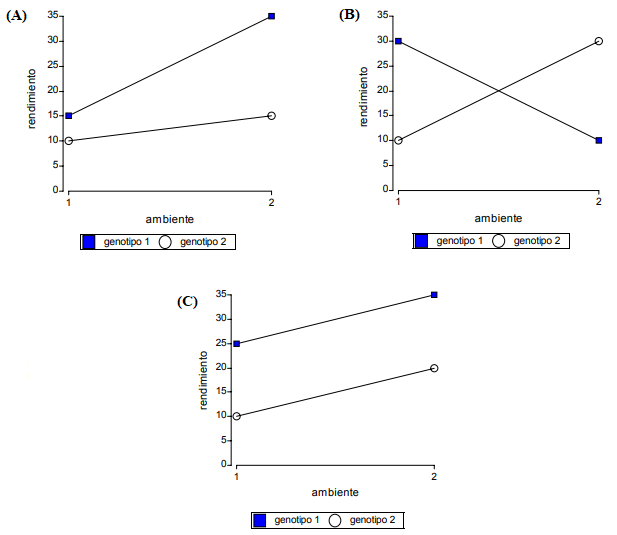
\includegraphics[width=14cm]{./Graficos/figura1}
\end{center}
\caption{Representación gráfica de tipos de IGA: (A)IGA no crossover, (B) IGA crossover y (C) no IGA}
\end{figure}


Distintos conceptos como regiones ecológicas, ecotipos, mega-ambientes, adaptaciones de germoplasma tanto en sentido amplio (a través de los ambientes) como específico (para cada ambiente o grupos de ambiente particular) (Kang et al., 2004) se pueden analizar a partir de la interacción genotipo-ambiente (Yan y Hunt, 2001).


Un análisis adecuado de la información de los EMA es indispensable para que el programa de mejoramiento de los cultivos sea eficaz. El rendimiento medio en los ambientes es un indicador suficiente del rendimiento genotípico solo en ausencia de IGA (Yan y Kang, 2003). Sin embargo, la aparición de IGA es inevitable y no basta con la comparación de las medias de los genotipos, sino que se debe recurrir a una metodología estadística más aporopiada. La metodología estadística más difundida para analizar los datos provenientes de EMA se basa en modificaciones de los modelos de regresión, análisis de variancia (\emph{Analysis of Variance}, ANOVA) y técnicas de análisis multivariado. 


Particularmente, para el estudio de la interacción y los análisis que de ella se derivan, dos modelos multiplicativos han aumentado su popularidad entre los fitomejoradores como una herramienta de análisis gráfico: el modelo de los efectos principales aditivos y interacción multiplicativa (AMMI, \emph{Additive Main effects and Multiplicative Interaction}) (Kempton 1984, Gauch, 1988), y el de regresión por sitio (SREG) (Cornelius et al., 1996; Crossa y Cornelius, 1997 y 2002).  Estos modelos combinan el análisis de varianza (ANOVA) y la descomposición de valores singulares (SVD) o el análisis de componentes principales (PCA) en la matriz residual de ANOVA. En SREG, el ANOVA se realiza sobre el efecto principal de A mientras que en AMMI se considera el efecto de G y A. A través del modelo AMMI se obtiene el gráfico biplot GE el cual es usado para explorar patrones puramente atribuibles a los efectos GE. Para el modelo SREG, Yan y Hunt (2002), presentaron la técnica GGE biplot usado para explorarnsimultáneamente patrones de variación en la suma G+GE.

Una limitación importante de la mayoría de las propuestas de análisis provenientes de EMA es que requieren que el conjunto de datos este completo. Aunque los EMA están diseñados para que todos los genotipos se evalúen en todos los ambientes,  las tablas de datos genotipo x ambiente completas son poco frecuentes (no todos los genotipos se encuentran en todos los ambientes). Esto ocurre, por ejemplo, debido a errores de medición o causas naturales como, por ejemplo, la destrucción de plantas por animales, inundaciones o durante la cosecha, la incorporación de nuevos genotipos y a que otros se descartan por su pobre desempeño (Hill y Rosemberg, 1985). En estos casos, entre las posibles soluciones para tratar con una tabla de datos incompleta es (i) el uso de un subconjunto completo de datos, eliminando aquellos genotipos que tienen valores faltantes (Ceccarelli et al., 2007, Yan et al., 2011), (ii) completar datos faltantes con la media ambiental, o (iii) imputación de datos faltantes con valores estimados utilizando, por ejemplo, un modelo multiplicativo (Kumar et al., 2012). 

En este contexto, el análisis de datos provenientes de EMA requiere metodología estadística sofisticada cuyas rutinas informáticas se encuentran disponibles en programas desarrollados por diferentes empresas. Esto genera el inconveniente de tener que disponer de todos los programas necesarios para los distintos análisis, atender los requerimientos de formatos de datos usados por cada uno, y comprender los diversos tipos de salidas en las que se ofrecen los resultados obtenidos. Además, algunos procedimientos, especialmente aquellas metodologías recientes, no se encuentran dispobibles, y los costos de las licencias de dichos programas resultan muy elevados. De aqui surge la necesidad de disponer de algún software libre que contemple la mayoría de las rutinas necesarias para analizar los datos provenientes de EMA. Este problema, puede ser resulto a partir del software R. Se trata de un proyecto de software libre distribuido bajo los términos de la \emph{General Public Licence} (GNU) que surge como resultado de la implementación de uno de los lenguajes más utilizados en investigación por la comunidad estadística, el lenguaje S. A diferencia de los programas estadísticos utilizados frecuentemente, R no dispone de una interfaz gráfica lo cual genera dificultad en su uso para aquellos que no se encuentran familiarizados con el uso de un lenguaje de programación. Sin embargo, brinda mayores posibilidades en cuanto a la manipulación y análisis de los datos ya lw permite a los usuarios definir sus propias funciones y  pesonalizar el tipo de análisis que desean realizar. 

R forma parte de un proyecto colaborativo ya que promueve el hecho de que los usuario creen funciones y las ponga al alcance de toda la comunidad.  Sin embargo, como muchas veces no resulta sencillo reutilizar una función creada por algun usuario se ha introducido la posibilidad de crear paquetes (\emph{package}) o librerías. Estas son una colección de objetos creados y organizados siguiendo un protocolo fijo que garantiza un soporte mínimo para el usuario así como la ausencia de errores (de sintaxis) en la programación.

R cuenta con 14 paquetes básicos y 29 recomendados para su funcionamiento instalados automaticamente en él, como por ejemplo, \emph{base} o \emph{stats}. Dado que la comunidad de usuarios que programan en R ha ido creciendo notablemente en los últimos años y que muchos de ellos han ido proporcionando librerías, se cuenta con una gran cantidad de paquetes que extienden las funciones básicas de R. Entre ellos se encuentran, \emph{plyr}, \emph{lubridate}, \emph{reshape2} y \emph{stringr} para la manipulación de los datos; \emph{ggplot2} y \emph{rgl} para la visualización; \emph{knitr} y \emph{xtable} para la presentación de resultados; entre otros. La lista completa de los paquetes oficiales puede consultarse en CRAN\footnote{CRAN (Comprehensive R Archve Network) es el repositorio oficial de paquetes de R, el lugar donde se publican las nuevas versiones del programa, etc. Contiene la lista completa de paquetes oficiales. \url{https://cran.r-project.org/web/packages/available_packages_by_name.html}}. Además de los paquetes oficiales, existen otros que pueden instalarse desde repositorios como, por ejemplo, Github. Sin embargo, no es sencillo encontrar un paquete que puede ser útil para un determinado fin sino que se debe recurrir a varios de ellos para cumplir un determinado objetivo. 

Frecuentemente, los mejoradores utilizan programas que tienen una interfaz gráfica para realizar los análisis estadísticos deseados y no tienen un manejo fluido de un lenguaje de programación. En el año 2012 se creó el paquete \emph{Shiny} que permite desarrollar aplicaciones Web utilizando R, acercando la potencia de R a todo tipo de usuarios.

El objetivo del presente trabajo fue: (i) crear un paquete de R que incluya las funciones que permitan analizar los datos provenientes de EMA, incluyendo además metodología recientemente publicada que no se encuentra disponible en R; (ii) crear una interfaz gráfica, entre R y el usuario, mediante Shiny con el fin de poder realizar los análisis disponibles en el paquete creado sin necesidad de utilizar el lenguaje de programación.



{\Huge{Pensar en hacer algun comentario de R studio}}
%% Los cap'itulos inician con \chapter{T'itulo}, estos aparecen numerados y
%% se incluyen en el 'indice general.
%%
%% Recuerda que aqu'i ya puedes escribir acentos como: 'a, 'e, 'i, etc.
%% La letra n con tilde es: 'n.
\chapter{Objetivos}
%\setcounter{section}{1}
\section{Objetivo general}
 
Desarrollar un paquete de R para el análisis de datos provenientes de EMA y una interfaza gráfica a través de la aplicación web Shiny.


\section{Objetivos específicos}
\begin{itemize}
\item Mostrar un flujo de trabajo reproducible para la construcción de paquetes de R.
\item Programar e incluir en el paquete de R metodología para el análisis de datos provenientes de EMA recientemente publicada y no disponible en R.
\item Añadir en el paquete de R funciones ya existentes con modificaciones o agregados para favorecer su uso.
\item Desarrollar una aplicación web Shiny que sirva como interfaz gráfica para el paquete.
\item Publicar el paquete y la aplicación para su libre uso.
\end{itemize}


%% Los cap'itulos inician con \chapter{T'itulo}, estos aparecen numerados y
%% se incluyen en el 'indice general.
%%
%% Recuerda que aqu'i ya puedes escribir acentos como: 'a, 'e, 'i, etc.
%% La letra n con tilde es: 'n.



\chapter{Métodos}
%\setcounter{section}{1}
\section{Paquete de R}

%https://oscarperpinan.github.io/R/Paquetes.html 
Una librería o paquete (\emph{package}) es una colección de objetos creados y organizados siguiendo un protocolo fijo que garantiza un soporte mínimo para el usuario así como la ausencia de errores (de sintaxis) en la programación.

\section{Creación del paquete de R}
Los pasos necesarios para la creación de un paquete son:
\begin{itemize}
\item Creación de los objetos que contendrá el paquete (funciones y/o
datos).
\item Creación del esqueleto del paquete.
\item Redacción de la documentación.
\item Compilación del paquete en Linux y creación de la versión para Windows.
\item Instalación.
\item Prueba y publicación.
\end{itemize}

\subsection{Objetos del paquete}
Un paquete puede contener cualquier tipo de objetos de R : funciones, datos etc. Lo primero que debe hacerse es programar las funciones y preparar los datos. El proceso de creación vigila que no hayan errores sintácticos pero no controla si hay errores lógicos.
 
\subsection{Esqueleto y estructura del paquete}
R proporciona una función \emph{package.skeleton} que permite automatizar el proceso de creación de un paquete creando los directorios, los archivos de documentación y otros objetos necesarios.
La  siguiente instrucción construye la estructura de un paquete llamado \emph{geneticae}, 

\begin{lstlisting}[frame=single]
package.skeleton(name = geneticae)
\end{lstlisting}

creando una carpeta de nombre \emph{geneticae} con 3 sub-carpetas en el directorio de trabajo y tres archivos sin extensión. Estos ultimos son los siguintes: 
\begin{itemize}

\item DESCRIPTION: contenido básico para
documentar según la descripción del paquete:

Package: geneticae\\
Type: Package\\
Title: What the package does (short line)\\
Version: 1.0\\
Date: 2019-09-21\\
Author: Who wrote it\\
Maintainer: Who to complain to <yourfault@somewhere.net>\\
Description: More about what it does (maybe more than one line)\\
License: What license is it under?\\

\item NAMESPACE: R usa un sistema de gestión de espacio de nombres que permite al autor del paquete especificar:
\begin{itemize}
\item las variables del paquete que se exportan (y son, por tanto, accesibles a los usuarios)
\item las variables que se importan de otros paquetes.
\item las clases y métodos S3 y S4 que deben registrarse.
\end{itemize}

Este mecanismo queda definido en el contenido del fichero NAMESPACE.

\item Read-and-delete-me: contiene algunas instrucciones importantes sobre cómo personalizar el paquete.
\end{itemize}

Las siguientes son las 3 sub-carpetas creadas:

\begin{itemize}
\item La carpeta \textbf{data} contiene todos los archivos correspondientes a los datos comprimidos con el nombre con el que fueron creados, con la extensión .rda. Estos no pueden ser modificados.
\item La carpeta \textbf{man} contiene todos los archivos de extensión .Rd y un archivo por objeto creado (datos o programa). Estos documentos son parte del sistema de ayuda del paquete en PDF y en HTML; por este motivo, la escritura sigue las reglas de LaTeX.
\item La carpeta \textbf{R} contiene todos los programas fuente, siendo .R la extensión de los mismos.
\end{itemize}
La documentación es uno de los aspectos mas importantes del código, sin ella, los usuarios no sabrán cómo usar el paquete. R proporciona una forma estándar de documentar paquetes: escribir archivos .Rd en la carpeta man, los cuales utilizan una sintaxis personalizada, basada en LaTeX. Sin embargo, el paquete \emph{roxygen2}, utilizado en este trabajo, permite obtener la documentación de una manera sencilla, proporcionando una serie de ventajas sobre la escritura los archivos .Rd:

\begin{itemize}
\item El código y la documentación son adyacentes, de modo que cuando el código se modifique, será fácil actualizar la documentación.

\item Inspecciona dinámicamente los objetos que está documentando, para que pueda agregar automáticamente los datos que de otra forma se deben escribir a mano.

\item Resume las diferencias en la documentación de los métodos S3 y S4, los genéricos y las clases, por lo que necesita aprender menos detalles.
\end{itemize}

Además de generar archivos .Rd, \emph{roxygen2} también creará un archivo NAMESPACE y administrará el campo \emph{Imports} del archivo DESCRIPTION.


\subsection{Compilación e instalación}
Una vez creada la documentación se debe chequear el paquete y generar los instaladores con su corresponiente manual. Para ello se utilizan las siguiente funciones:
\begin{itemize}
\item \emph{R CMD check} verificará que no haya errores de sintaxis o no se generen warnings. Está compuesto por más de 50 chequeos individuales entre los cuales se encuentran: la estructura del paquete, el archivo descripción, namespace, el código de R, los datos, la documentación, entre otros.
\item  \emph{R CMD build} compilará el paquete generando un archivo geneticae.tar.gz listo para su instalación en Linux y \emph{RCMD build -binary} generará el archivo para la instalación en Windows.
\item \emph{RCMD Rd2dvi --pdf} preparará el manual y \emph{R CMD INSTALL} instalará el paquete dejándolo listo para su uso
\end{itemize}

\subsection{Publicación}
%https://rsanchezs.gitbooks.io/ciencia-de-datos-con-r/paquetes/paquetes.html
Un repositorio es el lugar dónde están alojados los paquetes y desde el cuál se pueden descargarlos. Entre los repositorios más populares de paquetes R se encuentran:

\begin{itemize}
\item \textbf{CRAN}: es el principal repositorio de paquetes de R, está coordinado por la fundación R. Previa a la publicación en este repositorio el paquete debe pasar por diferentes pruebas para asegurar que cumple con las políticas de CRAN.

\item \textbf{Bioconductor}: se trata de un repositorio específico para bioinformática. Del mismo modo que CRAN, tiene sus propias políticas de publicaciones y procesos de revisión.

\item \textbf{GitHub}: a pesar que no es específico para R, github es con toda seguridad el repositorio más popular para la publicación de proyectos \emph{open source} (del inglés, código abierto). Su popularidad procede del espacio ilimitado que proporciona para el alojamiento de proyectos \emph{open source}, la integración con git (un software de control de versiones) y, la facilidad de compartir y colaborar con otras personas. Una de sus desventajas es que no proporciona procesos de control.

\item \textbf{R-Forge} y \textbf{RForge}: son entornos de desarrollo de paquetes y repositorios. Eso significa que incluyen control de fuente, seguimiento de errores y otras características. Puede obtener versiones de desarrollo de paquetes de estos.
\end{itemize}

El paquete \emph{geneticae} se encuentra en GitHub, para instalar el mismo (o cualquiera que se encuentre en dicho repositorio) se deben seguir las siguientes instrucciones:\\


\begin{lstlisting}[frame=single]
install.packages(remotes) 
library(remotes)
install_github(jangelini/geneticae) 
\end{lstlisting}


{\Huge{FALTAN LAS COMILLITAS EN INSTALL Y EN EL USUARIO DE GITHUB.. ME DA ERROR CUANDO LAS PONGO}}



{\Huge{(Ideas de: TRABAJO FINAL P SHINY)}}

\section{Aplicación Web}
Una aplicación web es una aplicación o herramienta informática accesible desde cualquier navegador, bien sea a través de internet (lo habitual) o bien a través de una red local. 
Estas aplicaciones son muy populares hoy en día para los usuarios no expertos, debido a la facilidad de su uso, ya que no es preciso instalar nada en el ordenador, simplemente se accede a través de un navegador. Además se puede acceder desde cualquier dispositivo con conexión a internet, ya sea un ordenador, un smartphone o una tablet, es decir que es independiente del sistema operativo del usuario. Otra gran ventaja es el bajo consumo de recursos, ya que la mayor parte del tiempo estos se consumen en el servidor donde se encuentra alojada la aplicación, que generalmente tiene mucha más potencia de cómputo que cualquier ordenador personal.

\section{Shiny APP}
%https://datanalytics.com/libro_r/shiny.html
Shiny es un paquete, que se encuentra instalado por defecto con Rstudio, con el que se pueden desarrollar aplicaciones web interactivas, directamente desde Rstudio sin necesitar conocimientos de HTML, CSS o Javascript. Shiny implementa la programación reactiva (cita de archivo aplicacion shiny) en donde los objetos (gráficos y tablas) que forman la aplicación responden a los inputs de los usuarios, dotando a estos de una gran capacidad de control.

En general, en estas aplicaciones, se distinguen tres pasos en el funcionamiento de la aplicación:
\begin{enumerate}
\item El usuario modifica todos aquellos widgets que quedan a su disposición en el navegador (los llamaremos inputs).
\item Los valores de los inputs se envían a R que realiza los análisis indicados.
\item Los resultados de estos cálculos se muestran en el navegador (los llamaremos outputs).
\end{enumerate}

El esquema interno de la aplicación puede observarse en la Figura \ref{fig:fig31}. 

\begin{figure}[h]
\begin{center}
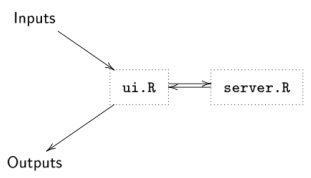
\includegraphics[width=7cm]{./Graficos/figura7}
\end{center}
\caption{Esquema interno de la aplicación.}
\label{fig:fig31}
\end{figure}


En las páginas y aplicaciones web se ha estandarizado el uso de ciertos lenguajes, tales como HTML, CSS, PHP o Javascript entre otros. Por defecto Shiny utiliza una plantilla básica de Twitter Bootstrap [18] para crear la interfaz de usuario, pero podemos descargar otras plantillas o crear una propia para personalizar nuestra aplicación. Twitter Bootstrap es un entorno de trabajo desarrollado por empleados de Twitter para fomentar la consistencia entre las herramientas internas, de forma que todas siguieran el mismo estilo. En 2011 Twitter liberó Bootstrap como código abierto, permitiendo que cualquiera lo usara para diseñar sus sitios o aplicaciones web. Contiene elementos de diseño basado en HTML, CSS y Javascript. Una de las mayores ventajas de Bootstrap es que permite crear interfaces web con CSS y JavaScript que adaptan la interfaz dependiendo del tamaño del dispositivo en el que se visualice de forma nativa, es decir, automáticamente se adapta al tamaño de un ordenador o de una tablet sin que el usuario tenga que hacer nada. Esto se denomina diseño adaptable o Responsive Design.

En lugar de usar un CSS propio para la interfaz de la aplicación se ha usado el paquete de R shinythemes [8], publicado por los creadores del propio Shiny. Shinytemes ofrece una serie de estilos básicos para aplicaciones Shiny.



\section{Creación de la Shiny APP}
%http://www.rpubs.com/JohanMarin/Shiny
La instalación de este paquete puede realizarse a través de los menús de Rstudio o simplemente con la siguiente orden:\\

\begin{lstlisting}[frame=single]
install.packages(shiny)
\end{lstlisting}

Para crear una Shiny app en \emph{File} se elige la opción Shiny Web App (figura \ref{fig:fig32}).

\begin{figure}[h]
\begin{center}
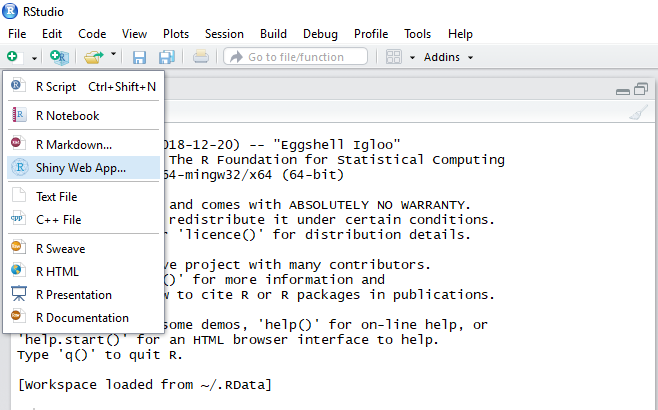
\includegraphics[width=12cm]{./Graficos/figura4}
\end{center}
\caption{Creación de Shiny Web App desde Rstudio}
\label{fig:fig32}
\end{figure}


Las aplicaciones Shiny están compuestas por un archivo app.R o dos archivos ui.R y server.R, es decir, se puede partir de un solo fichero que aglutine todo el código o se puede partir de dos archivos que separan la parte cliente de la parte servidora.

En este trabajo, se crea la aplicación Shiny mediante un unico script llamado app.R. El mismo se encuentra en un directorio (por ejemplo newdir/) y la aplicación se puede ejecutar con runApp(``newdir''). El script app.R esta formado por tres componentes:

\begin{itemize}
\item ui (\emph{user interfaz}): la interfaz de usuario controla el diseño de la aplicación, recibe los inputs y
muestra los outputs en el navegador.
\item server, funciones de R que contienen las instrucciones que se necesitan para construir los resultados de los análisis incluidos en la aplicación.
\item shinyApp, función que crea objetos de aplicación Shiny a partir de ui / servidor.
\end{itemize}


El archivo app.R deberá comenzar cargando el paquete Shiny y finalizar con una llamada a shinyApp:\\

\begin{lstlisting}[frame=single]
library(shiny)
ui<- ...
server<- ...
shinyApp(ui = ui, server = server)
\end{lstlisting}

La sesión de R estará monitoreando la aplicación y ejecutando las reacciones de la aplicación mientras la aplicación Shiny esté activa, por lo que no podrá ejecutar ningún comando.

La Figura \ref{fig:fig33} muestra el diseño utilizado en la aplicación. Se cuenta con un titulo y diferentes pestañas que conducen a diferentes páginas de la aplicación (\textbf{A}). Se cuenta con un panel de barra lateral (\textbf{B}), que contiene principalmente widgets con los cuales el usuario puede determinar el análisis que desea realizar y un panel principal (\textbf{C}) en el cual se obtenene los resultados del análisis solicitado.

\begin{figure}[h]
\begin{center}
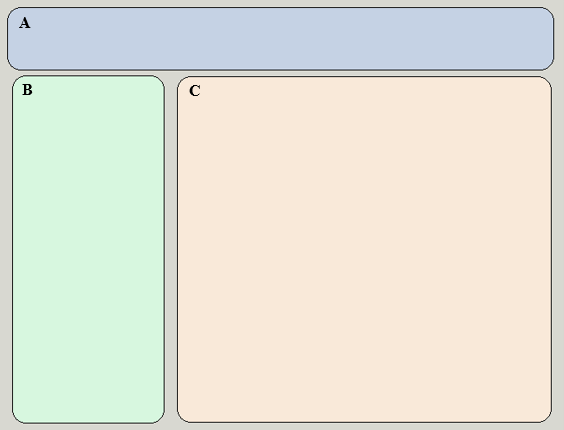
\includegraphics[width=12cm]{./Graficos/figura6}
\end{center}
\caption{Diseño de la aplicación Shiny. \textbf{A}: título y pestañas; \textbf{B}: área de entrada; \textbf{C}: área de resultados.}
\label{fig:fig33}
\end{figure}

\subsection{Tipos de componentes de Shiny Web App}

Los tipos de componentes de una aplación Shiny son:
\begin{itemize}
\item Componentes de Inputs y Outputs. Entre los inputs se encuentran numericInput, sliderInput, textInput, checkboxInput, entre otros. Posibles outputs se encuentran en la tabla \ref{tab:tabla1}, con las correspondientes funciones para server.R y ui.R
\item Componentes de Diseño. Algunos ejemplos se muestra en la tabla \ref{tab:tabla2}.
\item Componentes HTML (tags).
\end{itemize}


\begin{table}[h]
\begin{center}
\caption{Funciones para Outputs tanto para server.R como para ui.R}
\label{tab:tabla1}
\resizebox{\textwidth}{!} {
\begin{tabular}{cccc}
\hline
server.R & ui.R & espera & crea \\
\hline 
renderPlot & plotOutput & Gráfica & Gráfica\\
renderPrint & verbatimTextOutput, htmlOutput& salida impresa & texto\\
renderTable & tableOutput & objetos como tablas & tabla simple\\
renderDataTable & dataTableOutput & objetos como tablas & tabla DataTables.js\\
downloadHandler	& downloadButton, downloadLink & &\\
\hline 
\end{tabular}
}
\end{center}
\end{table}

\subsubsection{Componentes de Diseño}
% http://rstudio-pubs-static.s3.amazonaws.com/21373_8af3d3634b97461089c8a76659982915.html#componentes-shiny
\begin{itemize}
\item navbarPage(): Crea una página con una barra de navegación de nivel superior.
\item tabPanel(): Crea un panel de pestañas.
\item sidebarLayout(): Diseña de una barra lateral y el área principal.
\item sidebarPanel(): Crea un panel de barra lateral.
\item mainPanel(): Crea un panel principal.
\item navlistPanel(): Crea un panel de lista de navegación.
\item prettyRadioButtons(): Crea botones que permiten seleccionar un elemento de una lista.
\item materialSwitch(): Crea un interruptor de palanca para activar o desactivar una selección.
\item pickerInput(): Crea un control de selección de entrada.
\item navbarMenu():
\end{itemize}

{\small
\begin{table}[h]
\begin{center}
\caption{Componentes de Diseño de Shiny Web App}
\label{tab:tabla2}
\resizebox{0.6\textwidth}{!} {
\begin{tabular}{cccc}
\hline 
Componente	& Subcomponente	 \\
\hline
navbarPage(): & tabPanel(), navbarMenu()\\
navbarMenu() & tabPanel() \\
navlistPanel() & tabPanel()\\
titlePanel() &	\\
sidebarLayout() & sidebarPanel()  mainPanel() (obligatorio)	\\
sidebarPanel() & \\
mainPanel() & \\
tabsetPanel() &	\\
tabPanel()	 & \\
\hline
\end{tabular}
}
\end{center}
\end{table}
}


Para más información sobre estas componentes ver hoja de referencia de Shiny (Apéndice A).


\subsection{Compartiendo una Shiny Web App}

Una vez creada la aplicación, resulta conveniente ponerlas a disposición de los usuarios. En este caso la Shiny Web App encuentra disponible en el servidor de CONICET \url{www.cefobi.com}. Además el proyecto se encuentra en GitHub \url{https://github.com/jangelini/shinyAPP_geneticae}. 

%cambie un poco la estructura de resultados pero como para no reescribir la idea anterior le llame resultados 2
%% Los cap'itulos inician con \chapter{T'itulo}, estos aparecen numerados y
%% se incluyen en el 'indice general.
%%
%% Recuerda que aqu'i ya puedes escribir acentos como: 'a, 'e, 'i, etc.
%% La letra n con tilde es: 'n.


\chapter{Resultados}

\section{Paquete de R \emph{geneticae}}

Siguiendo el flujo de trabajo descripto en el capítulo anterior fue posible desarrollar el paquete de R \emph{geneticae} que implementa los métodos estadísticos discutidos para el análisis de datos de EMA.

El paquete \emph{geneticae} fue enviado a CRAN, donde pasó los exhaustivos controles de R CMD check exitosamente, logrando así una rápida aceptación  (\url{https://cran.r-project.
org/web/packages/geneticae/index.html}). En el momento de la escritura de este informe, pasaron 3 semanas desde su publicación en el repositorio y cuenta con más de 400 descargas, a pesar de que aún no se ha hecho difusión del paquete. El código fuente se encuentra disponible en GitHub (\url{https://github.com/
jangelini/geneticae}).

Para instalar la versión del paquete publicada en CRAN:  \textcolor{fandango}{install.packages(``geneticae")}, mientras que la versión en desarrollo se debe instalar desde el repositorio de GitHub:  \textcolor{fandango}{devtools::install\_github(``jangelini/geneticae")}. Una vez instalado el paquete, se debe cargar en la sesion de R mediante el comando: \textcolor{fandango}{library(geneticae)}. 

Información detallada sobre las funciones del paquete \emph{geneticae} se puede obtener mediante \textcolor{fandango}{help(package = ``geneticae")}. La ayuda para una función, por ejemplo \textcolor{fandango}{imputation()}, en una sesión R se puede obtener usando \textcolor{fandango}{?imputation} o \textcolor{fandango}{help(imputation)}. La función \textcolor{fandango}{browseVignettes(``geneticae")} permite obtener la viñeta del paquete, es decir una descripción el problema que está diseñado para resolver así como ejemplos de aplicación del mismo. 

Además, se encuentra disponible una página web que contiene una breve descripción de la utilidad del paquete, las funciones que se incluyen en él, un tutorial de uso, un enlace de acceso a la aplicación web Shiny, entre otros elementos (\url{https://jangelini.github.io/geneticae/}).


\subsection{Conjuntos de datos en \emph{geneticae}}
\label{subsec:datosejemplos}
El paquete \emph{geneticae} proporciona dos conjuntos de datos que pueden utilizarse para ilustrar la metodología incluida para analizar los datos provenientes de EMA. 

\begin{itemize}[wide, nosep, labelindent = 0pt, topsep = 1ex, noitemsep,topsep=0pt]
\item \emph{yan.winterwheat dataset} \citep{Wright2020}: cuenta con información sobre el rendimiento de 18 variedades de trigo de invierno cultivadas en nueve ambientes en Ontario en 1993. A pesar de que el experimento contaba con cuatro bloques o réplicas en cada ambiente, sólo el rendimiento medio para cada combinación de variedad y ambiente se encuentra disponible.\\

\begin{tcolorbox}[skin=bicolor,
    colframe=aurometalsaurus,colback=backcolour,colbacklower=white,
    width=1\linewidth,
    height=0.24\linewidth,
    boxsep=-3mm]
\begin{lstlisting}[linewidth=\columnwidth]
data(yan.winterwheat)
head(yanwinterwheat)[1:3,]
\end{lstlisting}

\tcblower\vskip-\baselineskip
\tcblower
\vspace{0.5cm}
\footnotesize\begin{verbatim}
##   gen  env yield
## 1 Ann BH93 4.460
## 2 Ari BH93 4.417
## 3 Aug BH93 4.669
\end{verbatim}
\end{tcolorbox}

\item \emph{plrv dataset} \citep{deMendiburu2020}: contiene información sobre el rendimiento, el peso de planta y de la parcela de 28 genotipos en 6 localidades de Perú. Cada clon fue evaluado tres veces en cada ambiente. \\

\begin{tcolorbox}[skin=bicolor,
    colframe=aurometalsaurus,colback=backcolour,colbacklower=white,
    width=1\linewidth,
    height=0.24\linewidth,
    boxsep=-3mm]
\begin{lstlisting}
data(plrv)
head(plrv)[1:3,]
\end{lstlisting}

\tcblower\vskip-\baselineskip
\tcblower
\vspace{0.5cm}
\footnotesize\begin{verbatim}
##   Genotype Locality Rep WeightPlant WeightPlot    Yield
## 1   102.18     Ayac   1   0.5100000       5.10 18.88889
## 2   104.22     Ayac   1   0.3450000       2.76 12.77778
## 3   121.31     Ayac   1   0.5425000       4.34 20.09259
\end{verbatim}
\end{tcolorbox} 
\end{itemize}
   
  
\subsection{Uso del paquete para ajustar el modelo AMMI}

Para visualizar el efecto de IGA se utiliza el biplot GE obtenido del modelo AMMI a través de la función \textcolor{fandango}{rAMMI()}, que requiere datos en formato largo, es decir, cada fila corresponde a una observación y cada columna a una variable (genotipo, ambiente, fenotipo observado y, si existe, repetición). Si cada genotipo ha sido evaluado más de una vez en cada ambiente, la media fenotípica para cada combinación de genotipo y ambiente se calcula internamente y luego se estima el modelo. El conjunto de datos puede contener variables adicionales no utilizadas en el análisis (a diferencia de lo que ocurre con muchos softwares y funciones de R disponibles hasta el momento). No se permiten valores perdidos pero se pueden imputar como se indica en la subsección \ref{subsec:metimp}. 

El primer argumento de \textcolor{fandango}{rAMMI()} es el conjunto de datos de entrada, luego se indican los nombres de las columnas en las cuales se encuentra la información necesaria para aplicar la técnica y por último el biplot que se desea obtener que por defecto es el derivado del modelo AMMI clásico. Opcionalmente, se puede agregar el porcentaje de IGA explicado por el biplot como una nota al pie mediante el argumento \emph{footnote = T} y un título con \emph{titles = T}. 

El biplot clásico para el conjunto de datos \emph{yan.winterwheat} se muestra en la figura
\ref{fig:ammibip}. En este ejemplo BH93, KE93 y OA93 son los ambientes que más contribuyen a la interacción ya que sus vectores son los de mayor magnitud. Los cultivares m12 y Kat presentan patrones de interacción similares (sus identificadores están próximos entre sí) y son muy diferentes de Ann y Aug, por ejemplo. La cercanía entre el cultivar Dia y el ambiente BH93 indica una fuerte asociación positiva entre ellos, lo que significa que BH93 es un ambiente extremadamente favorable para ese genotipo. Como los marcadores OA93 y Luc son opuestos, este ambiente es considerablemente desfavorable para ese genotipo. Por último, Cas y Reb están cerca del origen, lo que significa que se adaptan en igual medida a todos los ambientes.

\begin{tcolorbox}[skin=bicolor,
    colframe=aurometalsaurus,colback=backcolour,colbacklower=white,
    width=1\linewidth,
    height=0.82\linewidth,
    boxsep=-3mm]
\begin{lstlisting}
rAMMI(yan.winterwheat, genotype = ``gen", environment = ``env", 
      response = ``yield", type = ``AMMI", footnote = F, titles = F)
\end{lstlisting}
\tcblower\vskip-\baselineskip
\tcblower
\begin{figure}[H]
	\begin{center}
		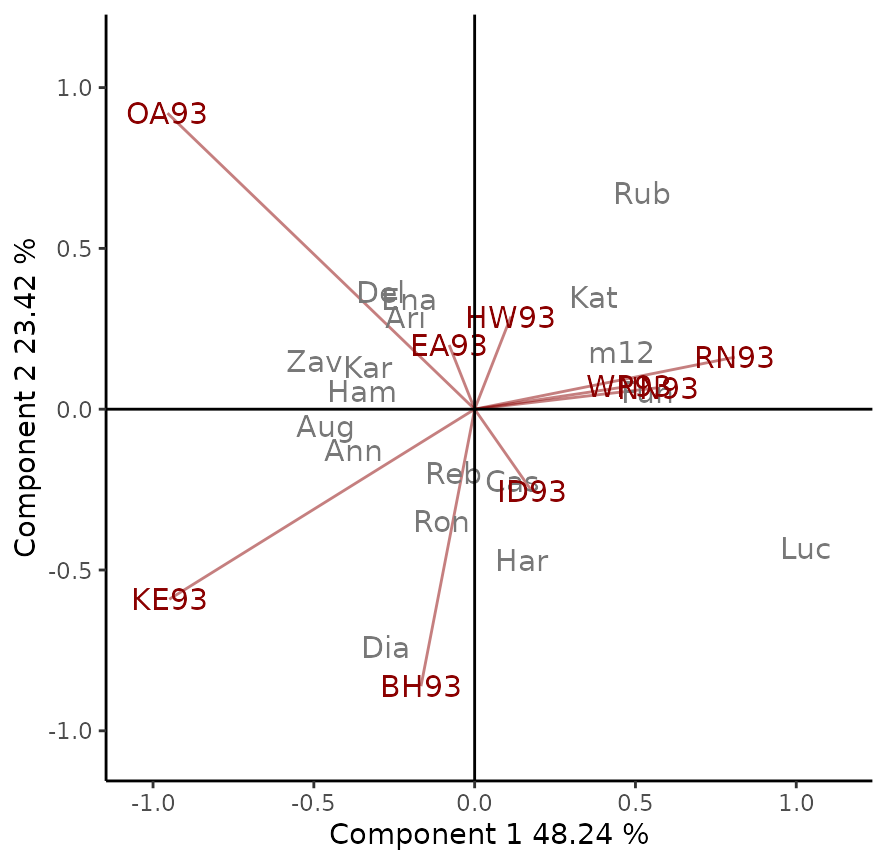
\includegraphics[width=0.50\textwidth]{./Graficos/AMMI_biplot.png}
	\end{center}
	\caption{Biplot GE obtenido del modelo AMMI clásico basado en los datos de rendimiento de trigo de invierno obtenidos en Ontario en 1993. El 71,66\% de la variabilidad de la IGA se explica por los dos primeros términos multiplicativos. Los cultivares se muestran en letras minúsculas y los ambientes en mayúsculas. }
	\label{fig:ammibip}
\end{figure}
\end{tcolorbox}


Como se mencionó anteriormente, el modelo AMMI, en su forma estándar, asume que no hay valores atípicos en los datos. Por lo tanto, en presencia de \emph{outliers} se debe utilizar alguna de las alternativas robustas propuestas por \citet{Rodriguesetal2016}, las cuales no se encuentran disponibles en R hasta el momento. Sin embargo, dada la importancia práctica de este reciente avance metodológico, se incluyeron en la función \textcolor{fandango}{rAMMI()}. Para obtener los biplots GE derivados de los modelos robustos se debe indicar en el argumento \emph{type} cuál de ellos se desea ajustar: ``rAMMI", ``hAMMI", ``gAMMI", ``lAMMI" o ``ppAMMI".

Dado que el conjunto de datos de muestra \emph{yan.winterwheat} no presenta valores atípicos, las conclusiones obtenidas con biplots robustos no difieren de las obtenidas con el biplot clásico \citep{Rodriguesetal2016}. Por lo tanto, no se presenta ninguna interpretación de los biplots robustos. 


\subsection{Uso del paquete para ajustar el modelo SREG}
\label{subsec:SREGpaquete}
Con el fin de visualizar conjuntamente el efecto de G e IGA \citet{Yanetal2000} propuso el biplot GGE mediante el cual se pueden abordar diversos aspectos relacionados con la evaluación de genotipos y ambientes. Para obtener dicho biplot en primer lugar se debe ajustar el modelo SREG mediante \textcolor{fandango}{GGEmodel()} que, del mismo modo que \textcolor{fandango}{rAMMI()}, requiere datos en formato largo. Si bien esta función invoca a \textcolor{fandango}{GGEModel()} del paquete \emph{GGEBiplots} \citep{Dumble2017}, al ser utilizada mediante \emph{geneticae} se permiten repeticiones y variables adicionales en el conjunto de datos. El rasgo fenotípico para cada combinación de genotipo y ambiente debe estar registrado, sino se debe recurrir previamente a alguna técnica de imputación para completar los datos (subsección \ref{subsec:metimp}). 

Se presenta a continuación la sentencia utilizada para ajustar el modelo SREG para el conjunto de datos \emph{yan.winterwheat}.

\begin{center}
\begin{tcolorbox}[colframe=aurometalsaurus,colback=backcolour,colbacklower=white,
   				width=1\linewidth,
    			height=0.08\linewidth,
    			boxsep=-3mm]
\begin{lstlisting}
GGE1 <- GGEmodel(yan.winterwheat, genotype = ``gen", environment = ``env",  response = ``yield", rep = NULL,  centering = ``tester", scaling = ``none",  SVP = ``symmetrical")
\end{lstlisting}
\end{tcolorbox}
\end{center}

El primer argumento es el nombre del conjunto de datos y en los siguientes se indican los nombres de las columnas que contienen la información de los genotipos, ambientes y del rasgo fenotípico de interés. Por defecto, la función considera que no hay réplicas en el conjunto de datos, sin embargo, si existieran en el parámetro \emph{rep} se debe indicar el nombre de la columna con dicha información. Otros argumentos son el método de centrado, de partición de los valores singulares (SVP por sus siglas en inglés, \emph{Singular Value Partition}) y escalado. Por defecto los datos se centran utilizando la opción \emph{centering=``tester"} lo cual resulta en el modelo SREG. La elección del método de SVP no altera las relaciones o interacciones relativas entre los genotipos y los ambientes, aunque la apariencia del biplot será diferente \citep{Yan2002}. El método de partición de los valores singulares centrado en los genotipos (\emph{SVP=``row"}) muestra la interrelación entre genotipos con mayor precisión, el enfocado a los ambientes (\emph{SVP=``column"}) es el más informativo de las interrelaciones entre los ambientes, mientras que el simétrico (\emph{SVP=``symmetrical"}) permite visualizar la magnitud relativa tanto de la variación de los genotipos como de los ambientes, por lo que se utiliza por defecto. Por último, se indica que los datos no se deben escalar con el parámetro \emph{scaling=``none"}. 

La salida de \textcolor{fandango}{GGEModel()} es una lista con los siguientes objetos:
\begin{itemize}
\item \emph{coordgenotype}: coordenadas para los genotipos en cada componente.
\item \emph{coordenviroment}: coordenadas para los ambientes en cada componente.
\item \emph{eigenvalues}: vector de autovalores para cada componente.
\item \emph{vartotal}: variancia general.
\item \emph{varexpl}: porcentaje de varianza explicado por cada componente.
\item \emph{labelgen}: nombres de los genotipos.
\item \emph{labelenv}: nombres de los ambientes.
\item \emph{axes}: etiquetas de los ejes.
\item \emph{Data}: datos escalados y centrados.
\item \emph{centering}: método de centrado.
\item \emph{scaling}: método de escala.
\item \emph{SVP}: método de partición. 
\end{itemize}


Utilizando la salida de \textcolor{fandango}{GGEmodel()}, la función 
\textcolor{fandango}{GGEPlot()} crea numerosas vistas del biplot GGE que permiten dar respuesta a distintos objetivos de los fitomejoradores. En estos gráficos los cultivares se muestran en minúsculas y los ambientes en mayúsculas. El método de centrado, escalado y SVP se muestran en una nota al pie junto con el porcentaje de G e IGA explicado por los dos ejes al agregar el argumento \emph{footnote = T} y un título con \emph{titles = T}. \\

\textbf{Comparaciones simples utilizando GGE biplot}

El biplot básico se obtiene con el parámetro \emph{type = ``Biplot"} (Figura \ref{fig:ggebip}). En este ejemplo, el 78\% de la variabilidad de G e IGA se explica por los dos primeros términos multiplicativos. Los ángulos entre los marcadores de genotipos y entre los vectores ambientales son utilizados para interpretar el gráfico. Así, por ejemplo, Kat tiene un rendimiento por debajo de la media en todos los ambientes debido a su ángulo superior a $90^{\circ}$ con todos ellos. Por otro lado, Fun presenta un rendimiento superior a la media en todas las localidades excepto OA93 y KE93, como lo indican los ángulos agudos. La longitud de los vectores ambientales es una medida de la capacidad del ambiente para discriminar entre cultivos. 


\begin{tcolorbox}[skin=bicolor,
    colframe=aurometalsaurus,colback=backcolour,colbacklower=white,
    width=1\linewidth,
    height=0.82\linewidth,
    boxsep=-3mm]
\begin{lstlisting}
GGEPlot(GGE1, type = ``Biplot", footnote = F, titles = F)
\end{lstlisting}
\tcblower\vskip-\baselineskip
\tcblower
\begin{figure}[H]
	\begin{center}
		\includegraphics[width=0.50\textwidth]{./Graficos/GGE_biplot.png}
	\end{center}
	\caption{Biplot GGE basado en datos de rendimiento de trigo de invierno obtenido de Ontario en 1993. El método de partición de valores singulares utilizado es el simétrico (opción por defecto). El 78\% de la variabilidad de G e IGA se explica por los dos primeros términos multiplicativos. Los cultivares se muestran en minúsculas y los entornos en mayúsculas. }
	\label{fig:ggebip}
\end{figure}
\end{tcolorbox} 


Con frecuencia, los mejoradores necesitan identificar los cultivares más adaptados a un ambiente particular, por ejemplo OA93. Para esto \citep{YanKang2003} sugieren construir un eje del ambiente de interés (OA93), trazando una recta que una el identificador del ambiente y el origen de coordenadas, y lo denominan eje OA93. Los genotipos se  clasifican en función del rendimiento en dicho ambiente de acuerdo con sus proyecciones, en la dirección indicada por el eje OA93 (Figura \ref{fig:selectEyG} (A)). Para obtener esta vista del biplot GGE, se indica la opción \emph{Selected Environment} en el argumento \emph{type} de la función y el ambiente a evaluar en el argumento  \emph{selectedE}. En este ejemplo, el cultivar de mayor rendimiento fue es Zav seguido por Aug, Ham hasta llegar al genotipo Luc, que es el de menor rendimiento en ese ambiente. El eje perpendicular al del ambiente de interés separa los genotipos con rendimiento mayor al promedio: de Zav a Cas, de aquellos con valores inferior a la media, de Ema a Luc, en OA93.
 
En forma similar, es posible determinar el ambiente más adecuado para un cultivar graficando una línea que conecte el origen de coordenadas y el marcador del genotipo de interés, por ejemplo Kat, como se muestra en la figura \ref{fig:selectEyG} (B) \citep{YanKang2003}. Los ambientes se clasifican a lo largo del eje del genotipo en la dirección indicada por la flecha. Para obtener este gráfico la opción  \emph{Selected Genotype} debe indicarse en el argumento \emph{type} y el genotipo de interés en \emph{selectedG}. El eje perpendicular al del genotipo separa los ambientes en los que el cultivar presentó un rendimiento por debajo y por encima del promedio. En este ejemplo, Kat presentó un desempeño por debajo de la media en todos los ambientes estudiados. \\

\begin{tcolorbox}[skin=bicolor,
    colframe=aurometalsaurus,colback=backcolour,colbacklower=white,
    width=1\linewidth,
    height=0.91\linewidth,
    boxsep=-3mm]
\begin{lstlisting}
# Ranking de cultivares en el ambiente OA93
GGEPlot(GGE1, type = ``Selected Environment", selectedE = ``OA93", footnote = F, titles = F)

# Ranking de ambientes para cultivar Kat
GGEPlot(GGE1, type = ``Selected Genotype", selectedG = ``Kat", footnote = F, titles = F)
\end{lstlisting}
\tcblower\vskip-\baselineskip
\tcblower
\begin{figure}[H]
	\begin{center}
		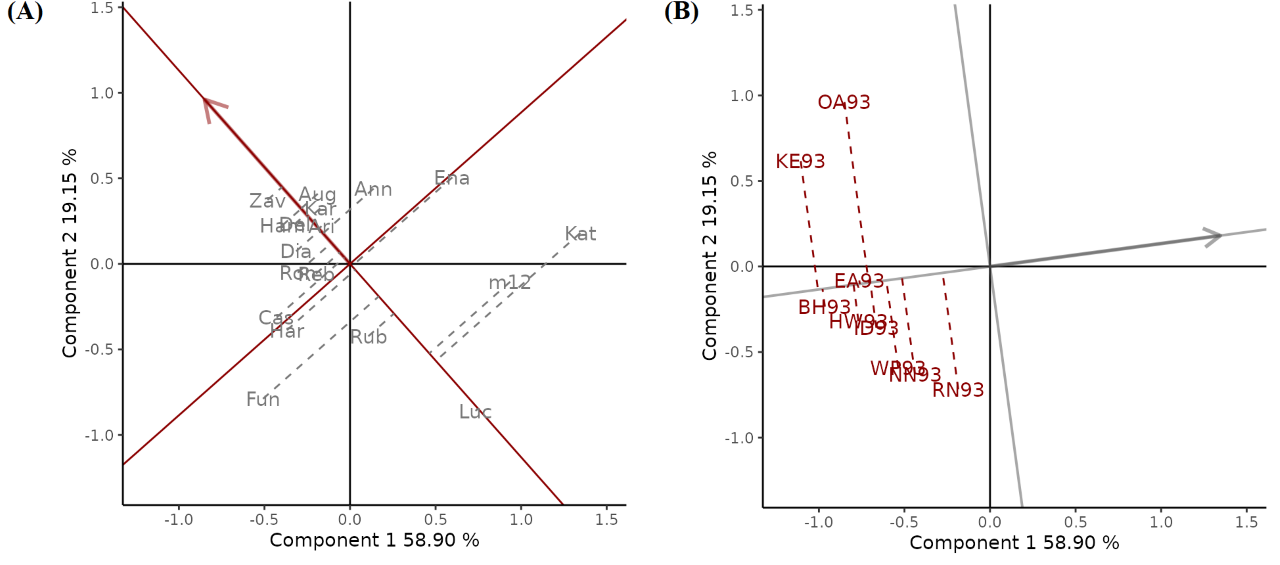
\includegraphics[width=0.95\textwidth]{./Graficos/SelectedGyE3.png}
	\end{center}
	\caption{ Ranking de (A) cultivares en el ambiente OA93 y (B) ambientes para cultivar Kat, basado en datos de rendimiento de trigo de invierno obtenido de Ontario en 1993. El método de partición de valores singulares utilizado es el simétrico (opción por defecto). El 78\% de la variabilidad de G e IGA se explica por los dos primeros términos multiplicativos. Los cultivares se muestran en minúsculas y los entornos en mayúsculas.}
	\label{fig:selectEyG}
\end{figure}
\end{tcolorbox} 


También es posible comparar dos cultivares, por ejemplo Kat y Cas, vinculándolos con una línea y trazando una recta perpendicular a ella (figura \ref{fig:comp2G}). Este biplot se obtiene con \emph{Comparison of Genotype} en el argumento \emph{type} y los genotipos a comparar en \emph{selectedG1} y \emph{selectedG2}. Cas fue más rendidor que Kat en todos los ambientes, ya que todos se ubican en el mismo lado de la línea perpendicular que Cas. \\

\begin{tcolorbox}[skin=bicolor,
    colframe=aurometalsaurus,colback=backcolour,colbacklower=white,
    width=1\linewidth,
    height=0.82\linewidth,
    boxsep=-3mm]
\begin{lstlisting}
GGEPlot(GGE1, type = ``Comparison of Genotype", selectedG1 = ``Kat", selectedG2 = ``Cas", footnote = F, titles = F)
\end{lstlisting}
\tcblower\vskip-\baselineskip
\tcblower
\begin{figure}[H]
	\begin{center}
		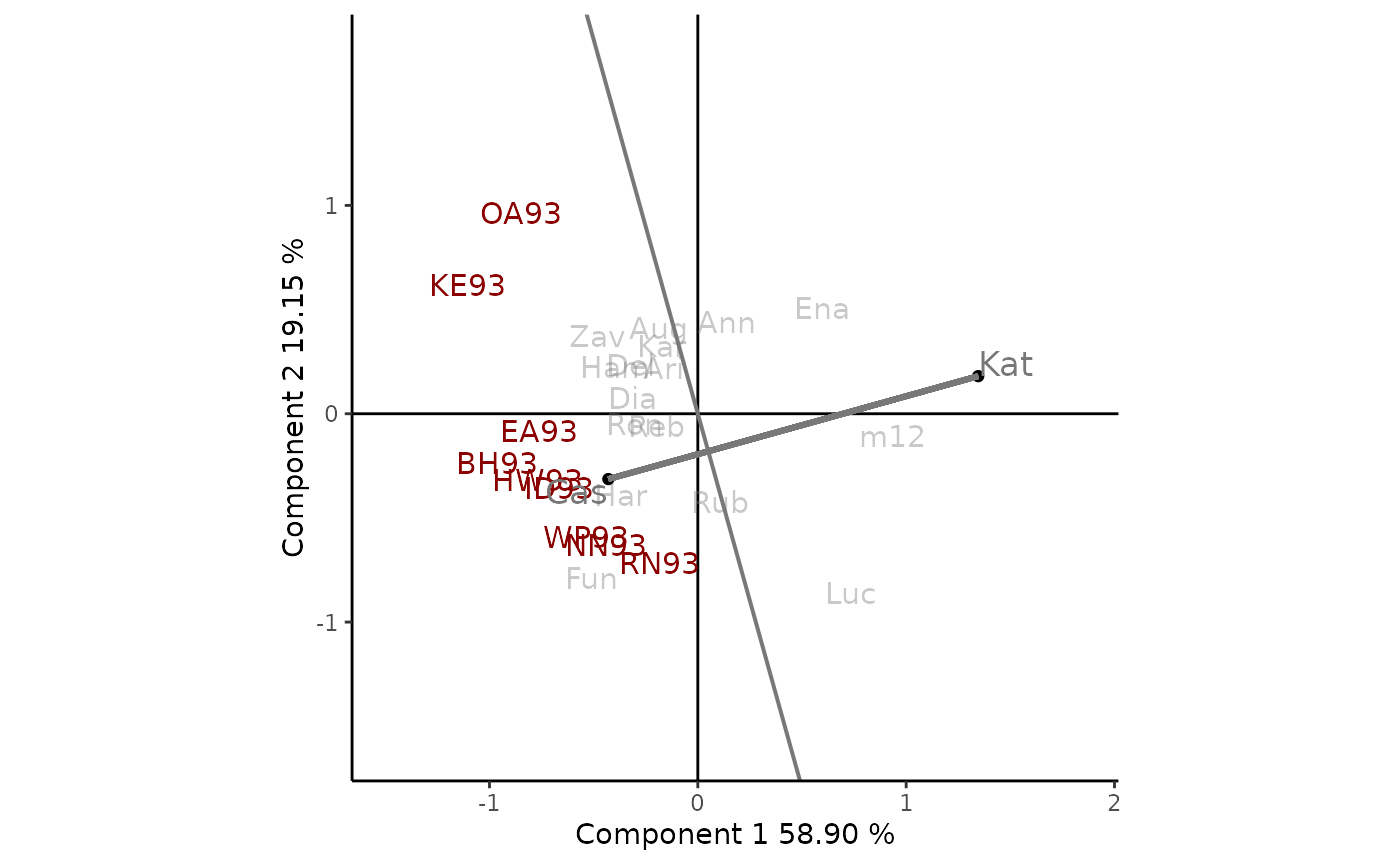
\includegraphics[width=0.50\textwidth]{./Graficos/GGE_comparisonG1yG2.png}
	\end{center}
	\caption{comparación de los cultivares Kat y Cas. El método de partición de valores singulares utilizado es el simétrico (opción por defecto). El 78\% de la variabilidad de G e IGA se explica por los dos primeros términos multiplicativos. Los cultivares se muestran en minúsculas y los entornos en mayúsculas. }
	\label{fig:comp2G}
\end{figure}
\end{tcolorbox}


\textbf{Identificación de mega-ambientes con GGE biplot}

La vista poligonal del biplot GGE, obtenida al indicar \emph{Which Won Where/What} en el argumento \emph{type}, proporciona un medio eficaz de visualización del patrón ``quíen ganó dónde"  de un conjunto de datos provenientes de EMA (Figura \ref{fig:poligono}).  El polígono se obtiene uniendo los cultivares (fun, zav, ena, kat y luc) que se encuentran más alejados del origen de coordenadas, de modo que todos los restantes se encuentren contenidos en el polígono. La distancia de los cultivares respecto del origen de coordenadas, en sus respectivas direcciones, es una medida de la capacidad de respuesta a los ambientes. Aquellos ubicados en los vértices son los más alejados, por lo tanto son los cultivares que más responden, mientras que los que se encuentran en el origen de coordenadas no responden en absoluto a los ambientes estudiados.

Las rectas perpendiculares a los lados del polígono dividen al biplot en mega-ambientes. El cultivar de mayor rendimiento en todos los ambientes de un mega-ambiente es el que se encuentra en el vértice del polígono. Por un lado, se observa que OA93 y KE93 conforman un mega-ambiente y que Zav es el mejor cultivar. El resto de los ambientes, forman otro mega-ambiente (identificado como ME1) siendo Fun el cultivar que se encuentra en el vértice. En el sector con ena, kat y luc en los vértices del polígono no se observó ningún ambiente, lo cual indica que estos cultivares fueron los menos rendidores en algunos o todos los ambientes considerados.\\

\begin{tcolorbox}[skin=bicolor,
    colframe=aurometalsaurus,colback=backcolour,colbacklower=white,
    width=1\linewidth,
    height=0.82\linewidth,
    boxsep=-3mm]
\begin{lstlisting}
GGEPlot(GGE1, type = ``Which Won Where/What", footnote = F, titles = F)
\end{lstlisting}
\tcblower\vskip-\baselineskip
\tcblower
\begin{figure}[H]
	\begin{center}
		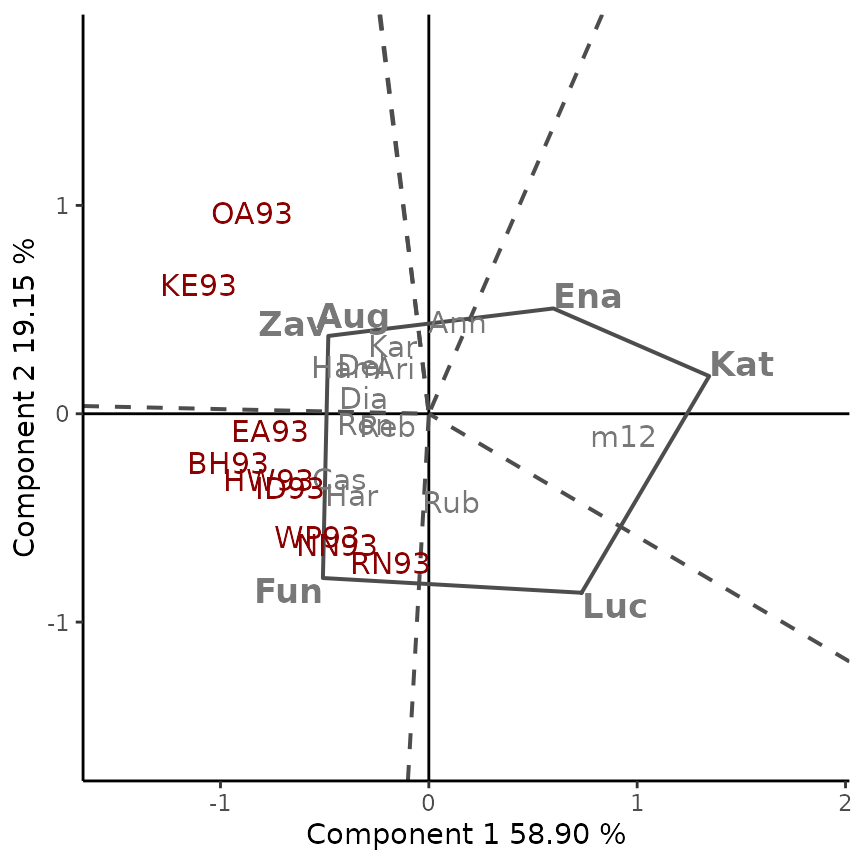
\includegraphics[width=0.48\textwidth]{./Graficos/GGE_whichwonwhere.png}
	\end{center}
	\caption{Vista poligonal del biplot GGE, que muestra qué cultivares presentaron mayor rendimiento en cada mega-ambiente. El método de partición de valores singulares utilizado es el simétrico (opción por defecto). El 78\% de la variabilidad de G e IGA se explica por los dos primeros términos multiplicativos. Los cultivares se muestran en minúsculas y los entornos en mayúsculas.}
	\label{fig:poligono}
\end{figure}
\end{tcolorbox}


\textbf{Evaluación de los cultivares dentro de un mega-ambientes con GGE biplot}

Una vez identificado los mega-ambientes, el siguiente paso es seleccionar cultivares dentro de cada uno de ellos. De acuerdo con la figura  \ref{fig:poligono}, zav es el mejor cultivar para los ambientes en uno de los mega-ambiente y fun para el otro. Sin embargo, los fitomejoradores generalmente no seleccionan un único cultivar en cada mega-ambiente, sino que evalúan a todos con el fin de conocer su desempeño (rendimiento y estabilidad).  

El biplot GGE, particularmente utilizando el factor de partición de la descomposición en valores singulares enfocando en los genotipos, es decir utilizando el argumento \emph{SVP=``row"} en la función \textcolor{fandango}{GGEmodel()}, proporciona un medio superior para visualizar tanto el rendimiento medio como la estabilidad de los genotipos. Esto se debe a que la unidad de ambos ejes para los genotipos es la unidad original de los datos. Además, dado que el interés radica en los genotipos y no en los ambientes, estos son omitidos del gráfico con el argumento \emph{sizeEnv = 0}.

La visualización del rendimiento medio y la estabilidad de los genotipos se logra dibujando una coordenada ambiental promedio (AEC, por sus siglas en inglés \emph{Average environment coordination}). Por ejemplo, la Figura \ref{fig:evaluacionG} (A)  muestra el AEC para el mega-ambiente ME1 compuesto por los entornos BH93, EA93, HW93, ID93, NN93, RN93 y WP93. La abscisa representa el efecto de G y la ordenada el de la IGA, que es una medida de la variabilidad o inestabilidad asociada con cada genotipo. Los cultivares se clasifican de acuerdo a su rendimiento medio a lo largo de la abscisa del AEC de acuerdo a la dirección de dicho eje, mientras que una proyección sobre la ordenada AEC muy alejada del origen, independientemente de la dirección, significa mayor inestabilidad. El cultivar de mayor rendimiento promedio en este mega-ambiente fue Fun, seguido por Cas y Har, mientras que Kat fue el de peor rendimiento medio. Rub y Dia son más variables y menos estables que otros cultivares, por el contrario, Cas, Zav, Reb, Del, Ari y Kar, fueron más estables. 

La Figura \ref{fig:evaluacionG} (B) compara los cultivares con uno considerado ``ideal” por ser el más rendidor y con estabilidad absoluta. Este cultivar ideal se usa como referencia, ya que rara vez existe. La distancia entre los cultivares y el ideal se puede utilizar como medida de conveniencia. Los círculos concéntricos ayudan a visualizar estas distancias. En el ejemplo, para el ME1, Fun es el más cercano al cultivo ideal, y por tanto el más deseable, seguido de Cas y Har, y Kat fue el más lejano. \\


\begin{tcolorbox}[skin=bicolor,
    colframe=aurometalsaurus,colback=backcolour,colbacklower=white,
    width=1\linewidth,
    height=1.05\linewidth,
    boxsep=-3mm]

\begin{lstlisting}

ME1 <- yan.winterwheat[yan.winterwheat(*@\$@*)env %in% c(``BH93", ``EA93",``HW93", ``ID93",``NN93", ``RN93", ``WP93"), ]
                                                   
# Modelo SREG enfocando SVD en los genotipos
GGE_Gpartition <- GGEmodel(ME1, genotype = ``gen", environment = ``env", response = ``yield", SVP = ``row")

# Visualizacion del rendimiento medio y la estabilidad
GGEPlot(GGE_Gpartition, type = ``Mean vs. Stability", footnote = F, titles = F, sizeEnv = 0)

# Ranking de los genotipos respecto a uno ideal
GGEPlot(GGE_Gpartition, type = ``Ranking Genotypes", footnote = F, titles = F, sizeEnv = 0)

\end{lstlisting}

\tcblower\vskip-\baselineskip
\tcblower
\begin{figure}[H]
	\begin{center}
		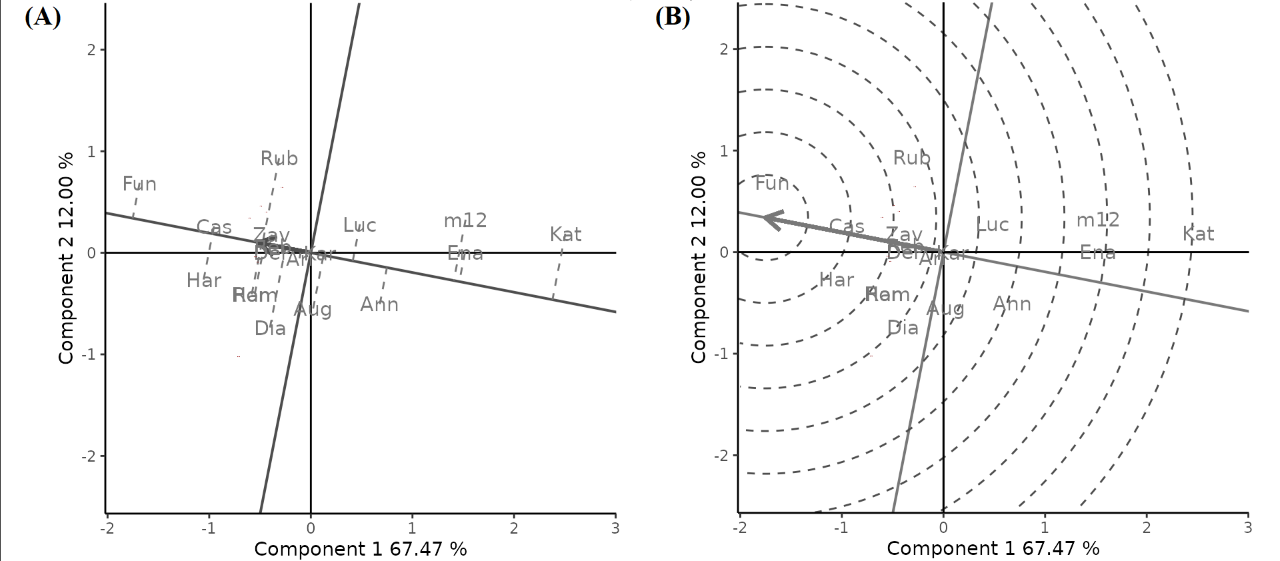
\includegraphics[width=0.90\textwidth]{./Graficos/MeanvsStability3.png}
	\end{center}
	\caption{(A) Evaluación de los cultivares con base en el rendimiento promedio y la estabilidad, y (B) clasificación de genotipos con respecto al genotipo ideal, basado en el método de partición de la descomposición en valores singulares enfocado en los genotipos.}
	\label{fig:evaluacionG}
\end{figure}
\end{tcolorbox}


\textbf{Evaluación de los ambientes con GGE biplot}

A pesar de que el objetivo principal de los EMA es seleccionar cultivares también es posible evaluar los ambientes. Esto incluye varios aspectos: (i) evaluar si la región objetivo pertenece a uno o más mega-ambientes; (ii) identificar mejores entornos de prueba; (iii) detectar ambientes redundantes que no brindan información adicional sobre cultivares; y (iv) determinar los ambientes que se pueden utilizar para la selección indirecta. Para ello, se enfoca la partición de los valores singulares en los ambientes al ajustar el modelo SREG (\emph{SVP = ``column"} en la función \textcolor{fandango}{GGEmodel()}). 

En la figura \ref{fig:evaluacionE} los ambientes están conectados con el origen de coordenadas a través de vectores, permitiendo comprender las interrelaciones entre ellos.  Esta visualización del biplot GGE se obtiene indicando \emph{Relationship Among Environments} (Figura \ref{fig:evaluacionE} (A)) en el parámetro \emph{type}. El coeficiente de correlación entre dos ambientes es aproximadamente el coseno del ángulo entre sus vectores. 
En este ejemplo se considera la relación entre los ambientes de ME1. El ángulo entre los vectores para los entornos NN93 y WP93 es de aproximadamente $10^{\circ}$ entre sus vectores; por lo tanto, están estrechamente relacionados; mientras que RN93 y OA93 presentan una correlación negativa débil ya que el ángulo es levemente mayor a $90^{\circ}$. El coseno de los ángulos no se traduce precisamente en coeficientes de correlación, ya que el biplot no explica toda la variabilidad en el conjunto de datos. Sin embargo, son lo suficientemente informativos como para comprender la interrelación entre los entornos de prueba. 

Si algunos de los ambientes tienen ángulos pequeños entre sí y, por lo tanto, están altamente correlacionados, la información sobre los genotipos obtenidos de estos ambientes debe ser similar. Si esta similitud se repite a través de los años, estos ambientes son redundantes y la evaluación de uno solo debería ser suficiente, permitiendo reducir costos en la experimentación.


La capacidad de discriminación así como la representatividad respecto del ambiente objetivo, son medidas fundamentales para un ambiente. Si no tiene capacidad de discriminación, no proporciona información sobre los cultivares y, por lo tanto, carece de utilidad. A su vez, si no es representativo no sólo que carece de utilidad sino que también puede proporcionar información sesgada sobre los cultivares evaluados. Para visualizar estas medidas, se define una coordenada ambiental promedio (AEC mencionado anteriormente) y el ambiente ideal como el centro de un conjunto de círculos concéntricos (Figura \ref{fig:evaluacionE} (B)). Para obtener este biplot se debe indicar \emph{Ranking Environments} en el argumento \emph{type} de \textcolor{fandango}{GGEPlot()}. El ángulo entre el vector de un ambiente y el eje proporciona una medida de la representatividad. Por lo tanto, EA93 e ID93 son los más representativos, mientras que RN93 y BH93 son los menos representativos del ambiente promedio, cuando se analiza ME1. Por otro lado, para ser discriminativo debe estar cercano al ambiente ideal. HW93 es el ambiente más cercano al ideal y, por lo tanto, es el más deseable del ME1, seguido por EA93 e ID93. Por el contrario, RN93 y BH93 fueron los ambientes de prueba menos deseables de ME1.  \\

\begin{tcolorbox}[skin=bicolor,
    colframe=aurometalsaurus,colback=backcolour,colbacklower=white,
    width=1\linewidth,
    height=0.89\linewidth,
    boxsep=-3mm]
\begin{lstlisting}
# Modelo SREG enfocando SVD en los ambientes
GGE_Epartition <- GGEmodel(ME1, genotype=``gen", environment=``env", response=``yield", SVP=``column")

# Relacion entre ambientes
GGEPlot(GGE_Epartition, type = ``Relationship Among Environments", footnote = F, titles = F)

# Clasificacion de ambientes con respecto al ambiente ideal
GGEPlot(GGE_Epartition, type = ``Ranking Environments", footnote = F, titles = F)
\end{lstlisting}
\tcblower\vskip-\baselineskip
\tcblower
\begin{figure}[H]
	\begin{center}
		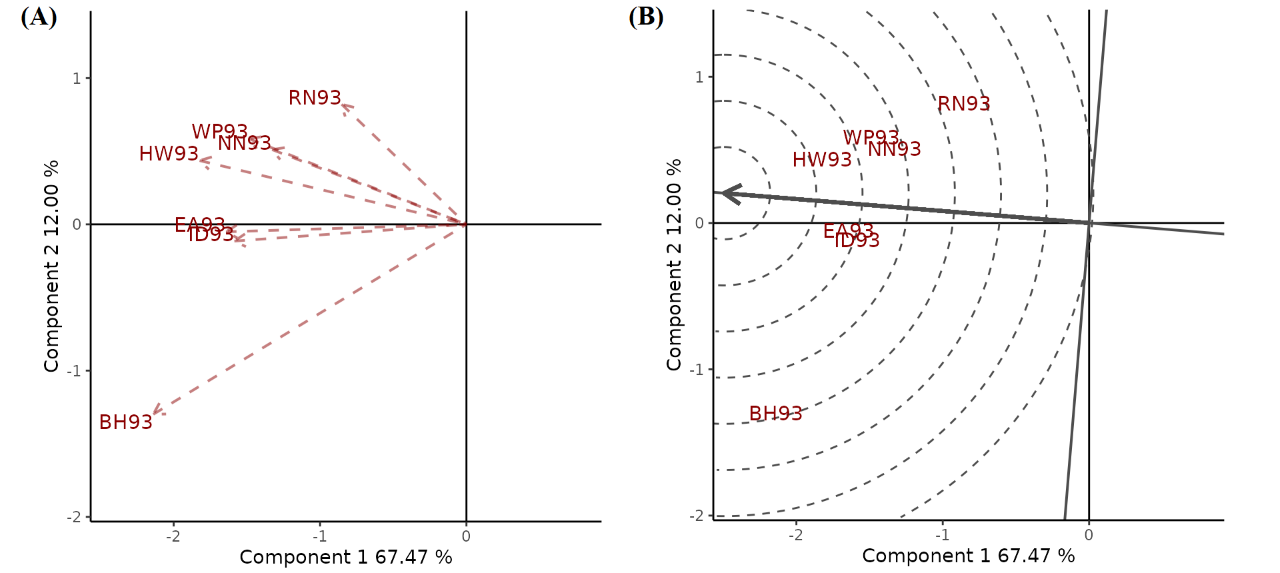
\includegraphics[width=0.90\textwidth]{./Graficos/RelationshipAmongEnvironments2.png}
	\end{center}
	\caption{(A) Relación entre ambientes y (B) clasificación de ambientes con respecto al ambiente ideal, basado en el escalado centrado en los genotipos.}
	\label{fig:evaluacionE}
\end{figure}
\end{tcolorbox}


\subsection{Uso del paquete para imputar matrices de datos incompletas}
\label{subsec:metimp}

Una limitación importante de los modelos presentados anteriormente es que requieren que el conjunto de datos este completo, es decir que todos los genotipos sean evaluados en todos los ambientes. Por lo tanto, en el paquete se incluyen una serie de metodologías de imputación desarrolladas específicamente para datos genotipo-ambiente recientemente publicadas, algunas de las cuales no se encuentran disponible en R, para superar el problema de las observaciones perdidas. Entre los métodos incluidos se encuentran: ``EM-AMMI", ``EM-SVD", ``Gabriel",``WGabiel''  y ``EM-PCA", los cuales se indican en la opción \emph{type} de la función \textcolor{fandango}{imputation()}. El formato requerido para el conjunto de datos de entrada es análogo al indicado en las otras funciones incluidas en el paquete. 

Para presentar un ejemplo, se eliminan algunas observaciones del conjunto de datos \emph{yan.winterwheat} ya que contaba con todos los registros completos:

\begin{tcolorbox}[skin=bicolor,
    colframe=aurometalsaurus,colback=backcolour,colbacklower=white,
    width=1\linewidth,
    height=0.15\linewidth,
    boxsep=-3mm]
\begin{lstlisting}
# Generando datos faltantes
yan.winterwheat [1,3] <- NA
yan.winterwheat [3,3] <- NA
yan.winterwheat [2,3] <- NA
\end{lstlisting}
\end{tcolorbox}

La imputación de valores perdidos con el método ``EM-AMMI" se puede realizar de la siguiente manera:

\begin{tcolorbox}[skin=bicolor,
    colframe=aurometalsaurus,colback=backcolour,colbacklower=white,
    width=1\linewidth,
    height=0.08\linewidth,
    boxsep=-3mm]
\begin{lstlisting}
imputation(yanwinterwheat, PC.nb = 2, genotype = ``gen", environment = ``env", response = ``yield", type = ``EM-AMMI")
\end{lstlisting}
\end{tcolorbox}

El resultado es la matriz con datos imputados en aquellas celdas vacías. 

\section{Aplicación web \emph{Geneticae}}

Siguiendo el procedimiento descripto se desarrolló la aplicación web \emph{Geneticae}, con el objetivo de proporcionar una interfaz gráfica de usuario para el paquete, de modo que pueda ser utilizado por fitomejoradores y analistas sin experiencia previa en programación R. El código fuente de \emph{Geneticae} se encuentra disponible en GitHub (\url{https://github.com/jangelini/Geneticae-Shiny-Web-APP}). 

Es un software interactivo, no comercial y de código abierto, que ofrece una alternativa gratuita al software comercial disponible para analizar datos provenientes de ensayos multiambientales. Momentáneamente se encuentra disponible en un servidor gratuito con una cuota mensual de horas de uso, al cual se puede acceder con el enlace \url{https://geneticae.shinyapps.io/geneticae-shiny-web-app/} o desde la página web \url{https://www.cefobi-conicet.gov.ar/bases-de-datos-y-programas/} del Centro de Estudios Fotosintéticos y Bioquímicos del Consejo Nacional de Investigaciones Científicas y Técnicas (CONICET).

A la brevedad la aplicación estará disponible para su uso ilimitado en los servidores del Centro de Cómputos del Centro Científico Teconológico (CCT) de Rosario, miembro del Sistema Nacional de Computación de Alto Desempeño. Como parte de este trabajo se solicitó al Centro de Cómputos la instalación de un \emph{Shiny Server}  (software que permite publicar este tipo de aplicaciones), habiendo resultado exitosa la publicación de una primera versión de prueba de \emph{Geneticae}. Actualmente, la versión final se encuentra en la cola de trabajo del equipo del CCT para su instalación definitiva y consiguiente apertura al público general.

En las subsecciones siguientes se presentará un ejemplo de cómo cargar y analizar datos con la aplicación web \emph{Geneticae}.

\subsection{Lectura de un archivo de datos para el uso de la aplicación web \emph{Geneticae}}

La aplicación web \emph{Geneticae} requiere que los datos de entrada se encuentren en archivos de texto plano, con delimitaciones por comas o punto y coma (formato .csv) o tabulaciones (formato .txt). Los nombres de las columnas pueden ubicarse en la primera fila del archivo (\emph{heading}). Los datos deben estar en formato largo, es decir, cada fila debe corresponder a una observación y cada columna a una variable (genotipo, ambiente, fenotipo observado y, si existe, repetición). Si cada genotipo ha sido evaluado más de una vez en cada ambiente, la media fenotípica requerida por el modelo SREG y AMMI para cada combinación de genotipo y ambiente se calcula internamente antes de ajustar dichos modelos. Las variables adicionales que no se utilizarán en el análisis pueden estar presentes en el conjunto de datos. No se permiten valores perdidos.

Los dos conjuntos de datos \emph{plrv} y \emph{yanwinterwheat} descriptos en la subsección \ref{subsec:datosejemplos} están disponibles en la pestaña \emph{Data $\rightarrow$ Example datasets} y se pueden descargar en formato .csv para poder seguir el tutorial de uso de la aplicación. El conjunto de datos \emph{yanwinterwheat} no tiene repeticiones, mientras que \emph{plrv} sí. 

En los siguientes ejemplos se trabajará con \emph{yanwinterwheat} para mostrar el uso de la aplicación. Luego de obtener el archivo de datos con el formato indicado, es posible importarlo en la pestaña \emph{Data $\rightarrow$ Upload data}. Por ejemplo, para importar \emph{yanwinterwheat}, se debe cargar el archivo .csv. Una vez cargado, se debe indicar que está delimitado por comas, que en la primera fila contiene los nombres de cada variable (\emph{heading}) y los nombres de las columnas en las cuales se encuentra la información del genotipo, ambiente y rasgo fenotípico (\emph{gen}, \emph{env} y \emph{yield} en este ejemplo) (Figura \ref{fig:fig431}). Si hay repeticiones disponibles, se debe especificar el nombre de la columna con dicha información; de lo contrario, el campo queda vacío. 

 \begin{figure}[h]
	\begin{center}
		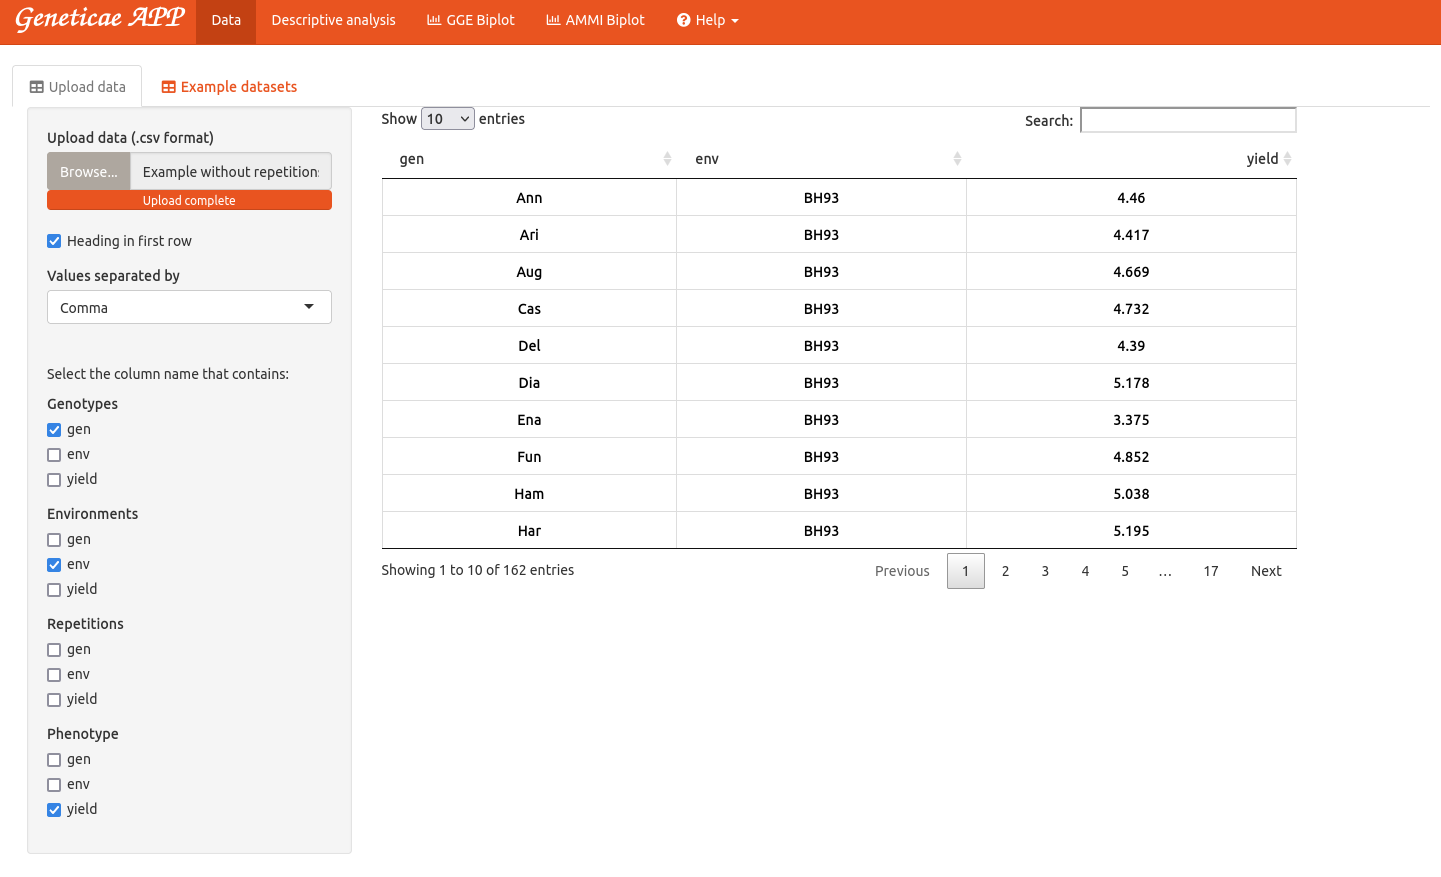
\includegraphics[width=0.9\textwidth]{./Graficos/www/Data.png}
	\end{center}
	\caption{Importar el conjunto de datos \emph{yanwinterwheat} en la aplicación web \emph{Geneticae}.}
	\label{fig:fig431}
\end{figure}

\hspace{1cm}

\subsection{Uso de la aplicación web \emph{Geneticae} para análisis descriptivo}

Cualquier estudio debe comenzar con un análisis descriptivo del conjunto de datos. La pestaña \emph{Descriptive Analysis} proporciona algunas herramientas para esto, como  \emph{boxplot}, diagrama y matriz de correlación y gráficos de interacción.

Un \emph{boxplot} que compara el rasgo cuantitativo entre ambientes o genotipos puede ser de interés (Figura \ref{fig:figdesc1}). Las medidas de resumen utilizadas para su construcción se muestran de forma interactiva moviendo el \emph{mouse} dentro del panel de la figura. Además, se puede descargar en formato .png o como un archivo interactivo .HTML, haciendo clic en la cámara que aparece en el gráfico o en el botón Descargar, respectivamente. El usuario puede personalizar algunos aspectos del gráfico, como el color de las cajas y los nombres de los ejes. 

\begin{figure}[h]
	\begin{center}
		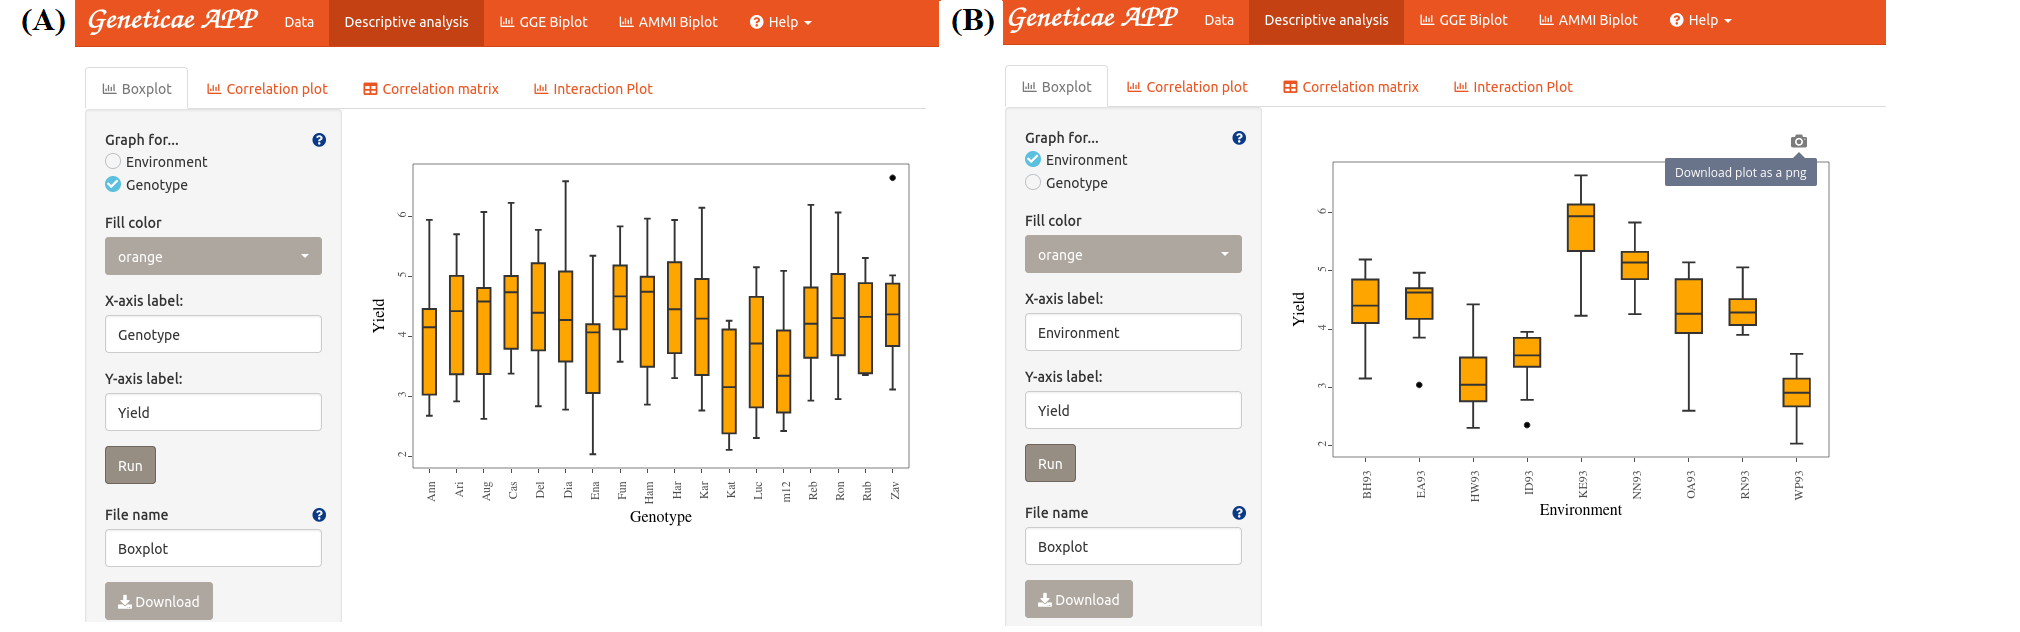
\includegraphics[width=0.95\textwidth]{./Graficos/www/boxplot.png}
	\end{center}
	\caption{Diagrama de caja de (A) genotipos y (B) ambientes para el conjunto de datos \emph{yanwinterwheat} obtenido con la aplicación web \emph{Geneticae}.}
	\label{fig:figdesc1}
\end{figure}


Los coeficientes de correlación de Pearson o Spearman entre genotipos se pueden mostrar con un gráfico o una matriz (Figura \ref{fig:figdesc2}). Gráficamente, las correlaciones positivas se muestran en azul y las negativas en rojo, mientras que la intensidad del color y el tamaño del círculo son proporcionales a la magnitud de los coeficientes de correlación. La gráfica de correlación se puede descargar en formato .png. En el ejemplo, se observan altas correlaciones entre el rendimiento de los genotipos estudiados. 

\begin{figure}[h]
	\begin{center}
		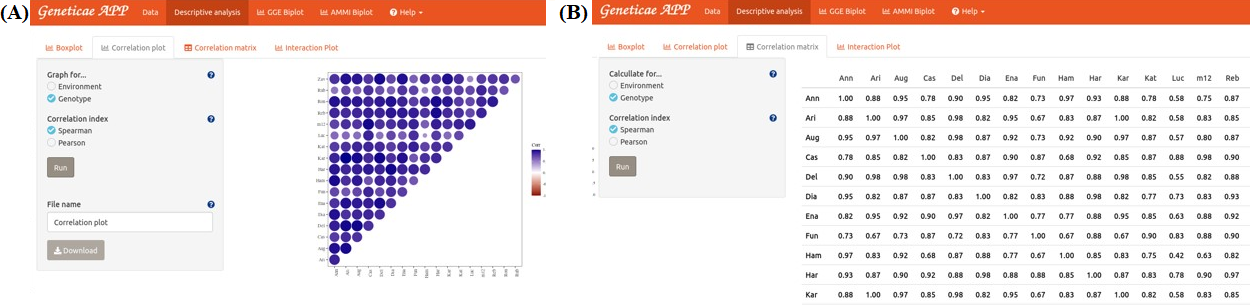
\includegraphics[width=0.95\textwidth]{./Graficos/www/correlacion.png}
	\end{center}
	\caption{(A) Gráfico y (B) matriz de correlación entre genotipos para el conjunto de datos \emph{yanwinterwheat} obtenido con la aplicación web \emph{Geneticae}.}
	\label{fig:figdesc2}
\end{figure}


Dado que la IGA genera respuestas genotípicas diferenciales en diferentes ambientes complicando la selección de los mejores cultivares, una gráfico de interacción puede ser de interés (Figura \ref{fig:figdesc3}). El cambio en el efecto genotípico a través de los ambientes se muestra en la figura \ref{fig:figdesc3} A, mientras que el cambio en el efecto ambiental a través de los genotipos en la figura \ref{fig:figdesc3} B. Estos también son gráficos interactivos por lo que es posible descargarla en formatos .HTML o .png con el botón Descargar o haciendo clic en la cámara que aparece en el gráfico, respectivamente. Además, el usuario puede personalizar los nombres de los ejes. En este ejemplo se pueden ver inconsistencias en el desempeño de genotipos en diferentes ambientes. 


\begin{figure}[h]
	\begin{center}
		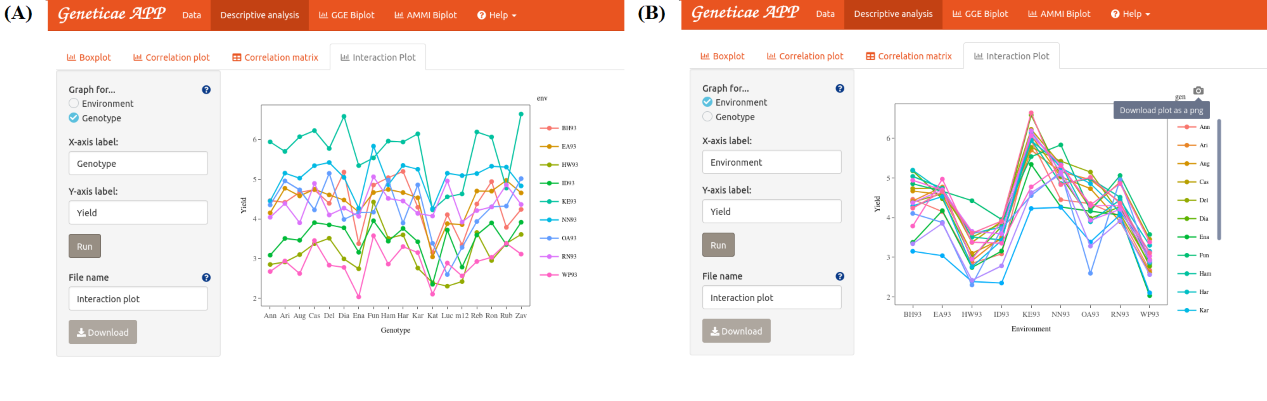
\includegraphics[width=0.95\textwidth]{./Graficos/www/interaction.png}
	\end{center}
	\caption{Gráfico de interacción para (A) ambientes a través de genotipos y (B) genotipos a través de los ambientes para conjunto de datos de \emph{yanwinterwheat} obtenido con la aplicación web \emph{Geneticae}.}
	\label{fig:figdesc3}
\end{figure}


\subsection{Uso de la aplicación web \emph{Geneticae} para ajustar el modelo SREG}

La aplicación web \emph{Geneticae} permite generar las vistas del biplot GGE presentados en la subsección \ref{subsec:SREGpaquete} mediante la pestaña \emph{GGE Biplot}. Del mismo modo que en el paquete \emph{geneticae}, los cultivares se presentan en minúsculas y los ambientes en mayúsculas. Dado que el modelo SREG requiere una única observación para cada combinación de genotipo y ambiente, si hay repeticiones, el valor fenotípico promedio se calcula automáticamente antes de ajustar el modelo. No se permiten valores perdidos. 

Se debe seleccionar el método de partición de los valores singulares (\emph{SVP type}). Como se mencionó anteriormente esta elección no altera las relaciones o interacciones relativas entre genotipos y ambientes, aunque la apariencia del biplot será diferente (Yan, 2002). La opción simétrica permite la comparación tanto de genotipos como de ambientes (opción por defecto); \emph{Genotype-Focused} muestra la interrelación entre genotipos con mayor precisión que cualquier otro método y \emph{Environment-Focused} es la que más informa sobre las interrelaciones entre ambientes. Una nota a pie del gráfico indica el método de centrado utilizado (para el biplot GGE siempre es \emph{tester-center}), el método SVP elegido por el usuario y que no se aplica ninguna escala a los datos. Además, se puede agregar el porcentaje de variabilidad de G e IGA explicado por las dos PC, mientras que la inclusión de títulos, ejes y etiquetas es opcional. Ciertos atributos estilísticos de dichos gráficos se pueden personalizar como el color y tamaño de los identificadores de los genotipos y de los ambientes. Los gráficos pueden ser descargados.  

El biplot básico, la vista del biplot GGE que muestra los cultivares más adecuados para un ambiente particular (OA93), los ambientes más adecuados para un genotipo (Kat), la comparación de dos genotipos (Cas y Kat) y la vista del poligono se pueden obtener como se indica en la figura \ref{fig:ggebip1}, donde el escalado es el simétrico (\emph{SVP type $\rightarrow$ symmetrical}) y las opciones de \emph{plot type} son \emph{Biplot,
Selected Environment, Selected Genotype, Comparison of Genotype} y \emph{Which Won Where/What}, respectivamente. Al indicar \emph{Selected Environment} el ambiente de interés se debe especificar, de igual modo cuando se utiliza \emph{Selected Genotype} y 
\emph{Comparison of Genotype} se debe señalar cuál es el genotipo a analizar.

\begin{figure}[H]
	\begin{center}
		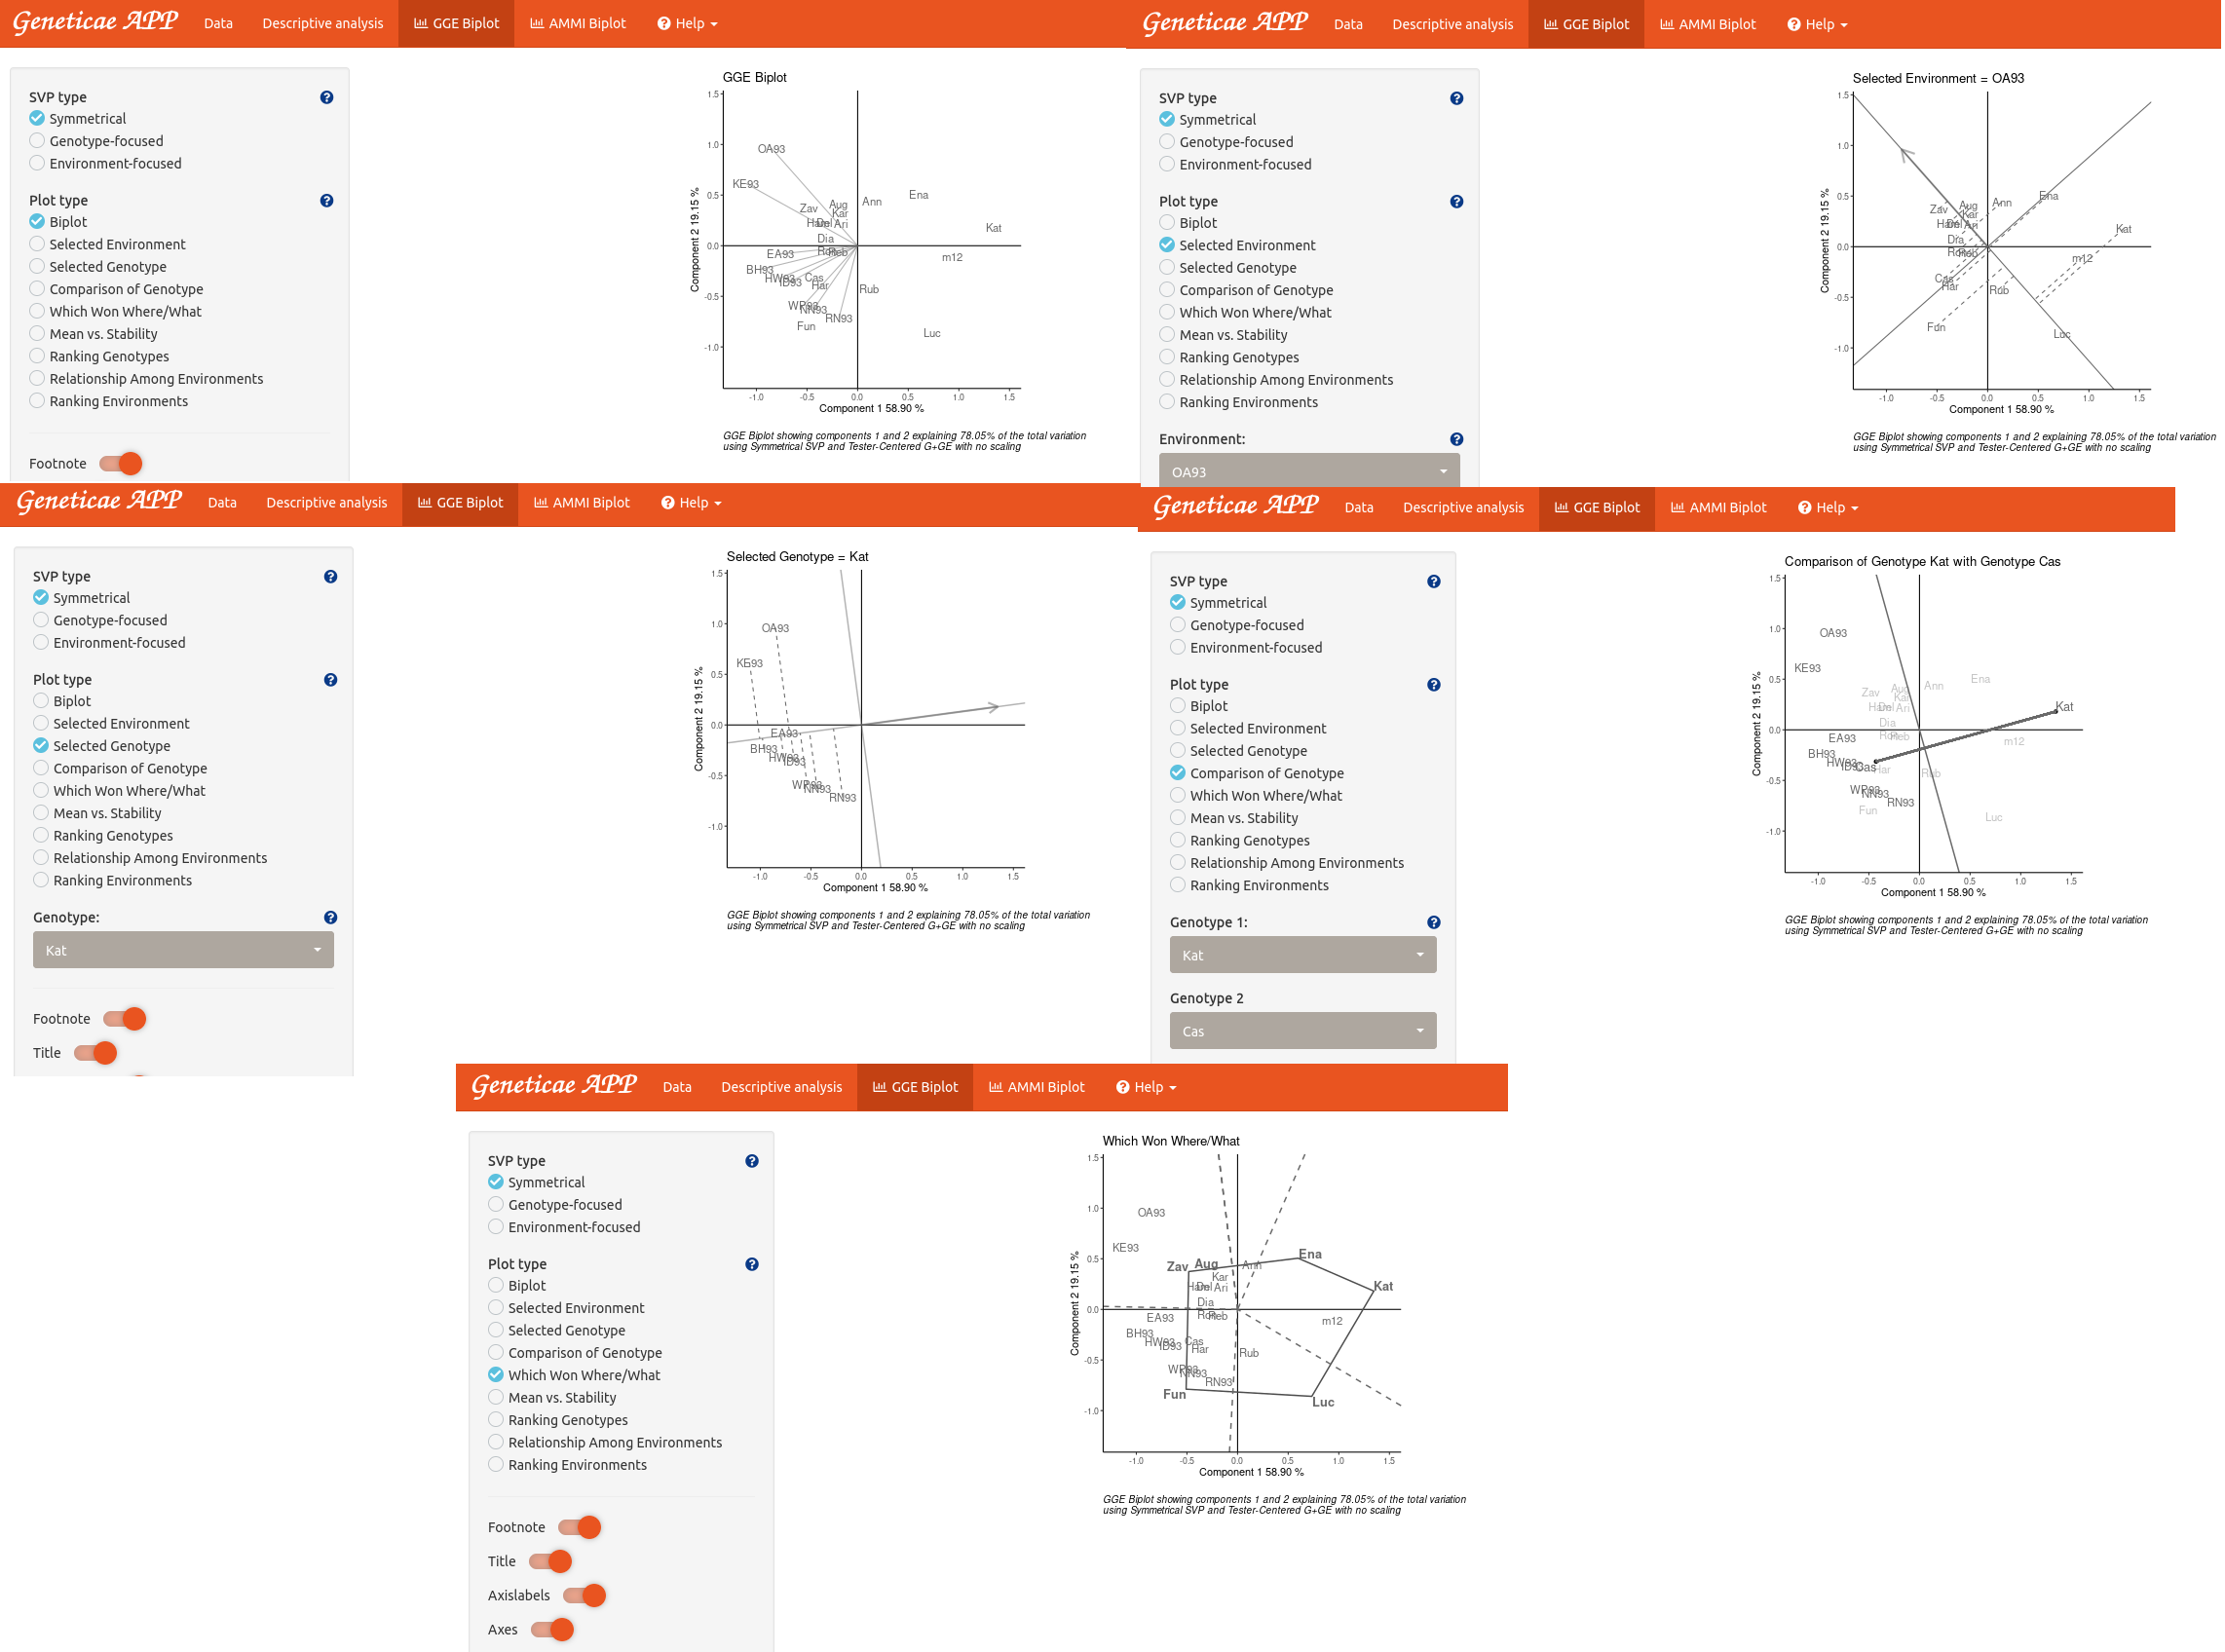
\includegraphics[width=0.9\textwidth]{./Graficos/www/GGE_biplotAPP1.png}
	\end{center}
	\caption{Vistas del biplot GGE usando la partición en valores singulares simétrica obtenidos con la aplicación web \emph{Geneticae}.}
	\label{fig:ggebip1}
\end{figure}

La selección de cultivares dentro de cada mega-ambiente se realiza con la partición de valores singulares enfocada en los genotypos (\emph{SVP type $\rightarrow$ genotype-focused}), y los tipos de gráficos que se pueden realizar son: \emph{Mean vs. Stability} que permite la visualización de la media y estabilidad de genotipos y \emph{Ranking Genotypes} que compara las cultivares con el ``ideal" (Figura \ref{fig:ggebip2}). Dado que estos análisis son propios de cada mega-ambiente, al indicar alguno de estas vistas del biplot GGE se tendrá que señalar cuales son los ambientes que forman el mega-ambiente de interés. 


\begin{figure}[h]
	\begin{center}
		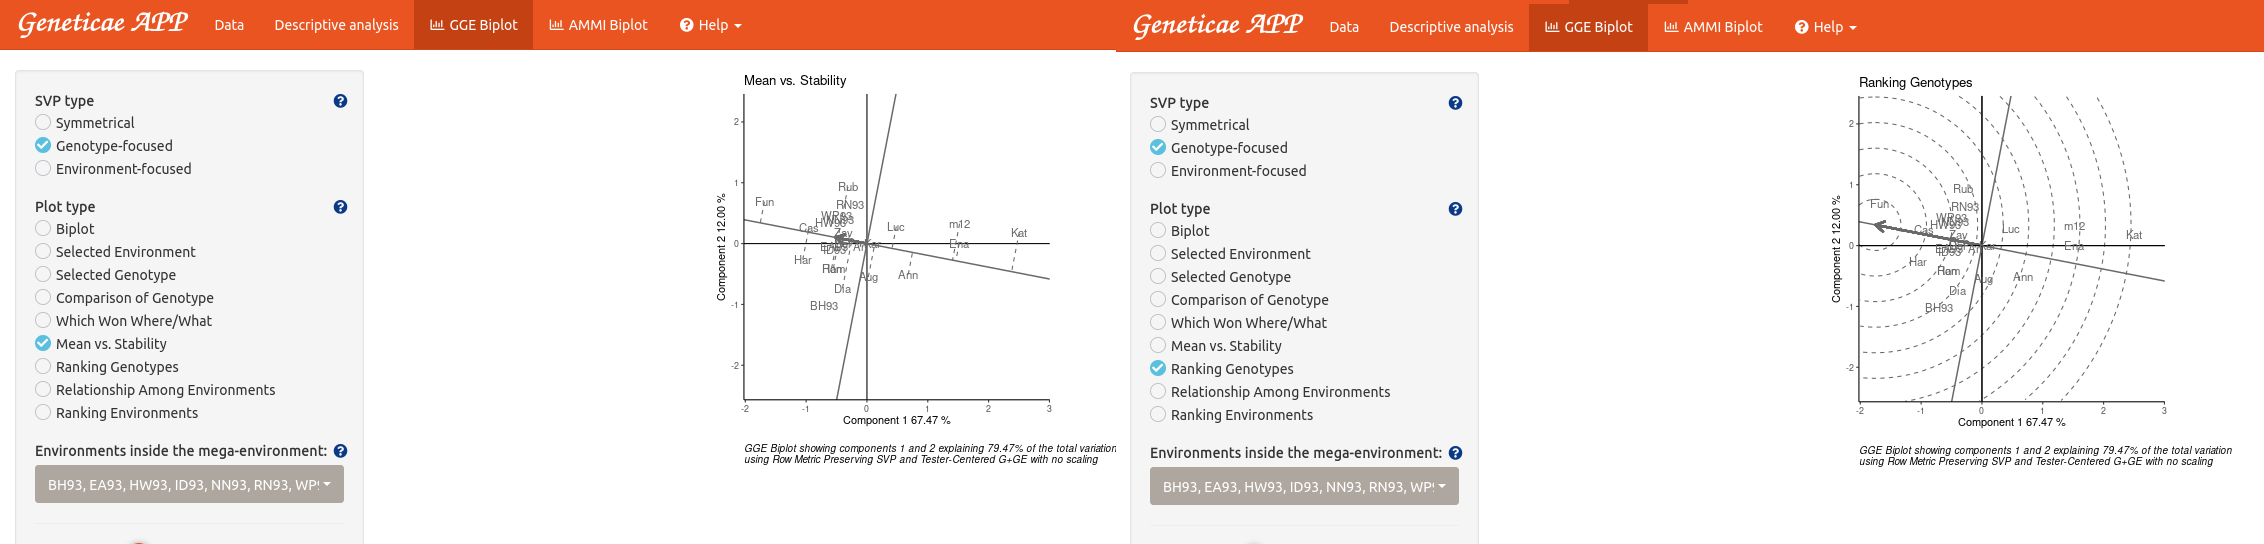
\includegraphics[width=0.95\textwidth]{./Graficos/www/GGE_biplotAPP2.png}
	\end{center}
	\caption{Vistas del biplot GGE usando la partición de valores singulares enfocada en los genotipos obtenidos con la aplicación web \emph{Geneticae}.}
	\label{fig:ggebip2}
\end{figure}

Por último, para el análisis de los ambientes de cada mega-ambiente se utiliza el método de partición de valores singulares centrado en los ambientes (\emph{SVP type $\rightarrow$ environment-focused}). El tipo de gráfico \emph{Relationship Among Environments} permite comprender la interrelación entre los ambientes, mientras que \emph{Ranking Environments} se utiliza para visualizar la capacidad de discriminación y representatividad (Figura \ref{fig:ggebip3}). Como en el caso anterior, al indicar alguna de estas vistas del biplot GGE se tendrá que señalar cuales son los ambientes que forman el mega-ambiente de interés. 


\begin{figure}[h]
	\begin{center}
		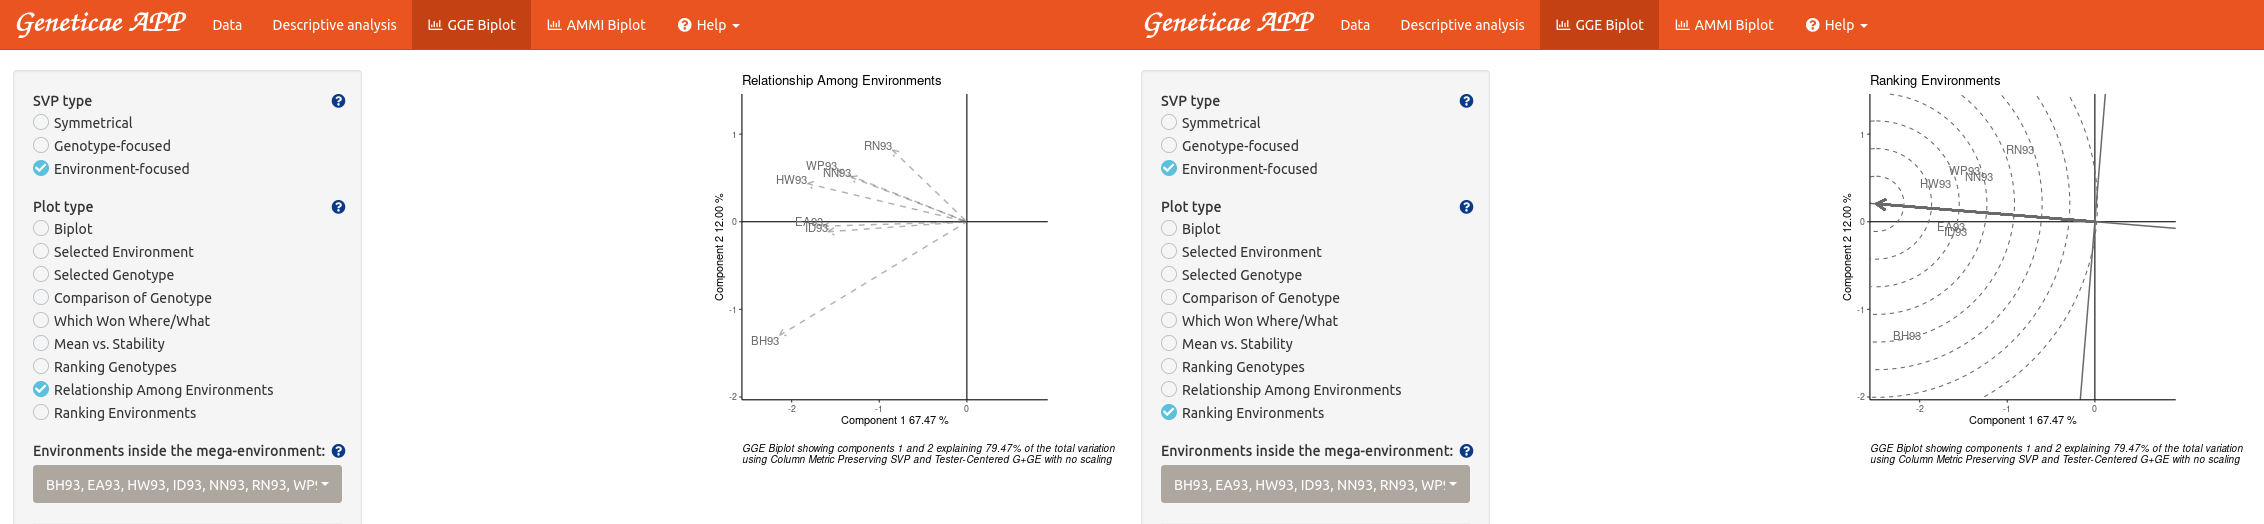
\includegraphics[width=0.95\textwidth]{./Graficos/www/GGE_biplotAPP3.png}
	\end{center}
	\caption{Vistas del biplot GGE usando la partición de valores singulares enfocada en los ambientes obtenidas con la aplicación web \emph{Geneticae}.}
	\label{fig:ggebip3}
\end{figure}


\subsection{Uso de la aplicación web \emph{Geneticae} para ajustar el modelo AMMI}

La pestaña \emph{AMMI Biplot} crea el biplot GE. Dado que las alternativas clásica y robustas requieren una única observación para cada combinación de genotipo y ambiente, si hay repeticiones, el valor promedio fenotípico se calcula automáticamente antes de ajustar el modelo. No se permiten valores perdidos. Como con las figuras anteriores, se ofrecen opciones de configuración y de descarga.

Por ejemplo, para obtener el biplot GE derivado del modelo AMMI clásico se debe indicar AMMI en \emph{plot type} (Figura \ref{fig:figammiapp}). En caso de contar con \emph{outliers}, alguna de las alternativas robustas (rAMMI, hAMMI, gAMMI, lAMMI o ppAMMI).
 

\begin{figure}[h]
	\begin{center}
		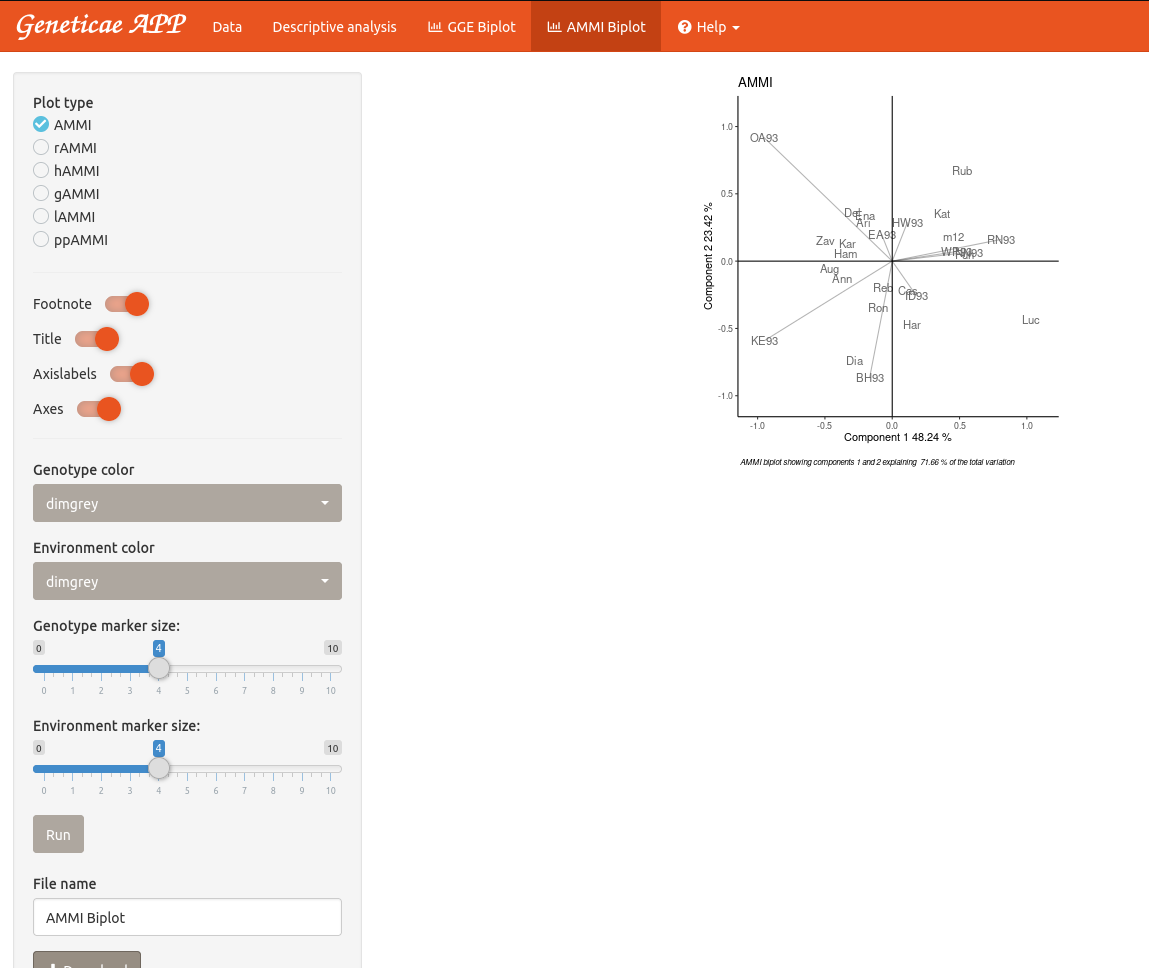
\includegraphics[width=0.70\textwidth]{./Graficos/AMMI_GE.png}
	\end{center}
	\caption{Biplot GE derivado del modelo AMMI clásico basado en datos de rendimiento de trigo de invierno obtenido de Ontario en 1993 obtenido con la aplicación web \emph{Geneticae}.}
	\label{fig:figammiapp}
\end{figure}


\subsection{Ayuda}

En la pestaña \emph{Help} se presenta información general, un tutorial y un video sobre cómo utilizar la aplicación web \emph{Geneticae}.

%\include{capitulo3}
\chapter{Conclusión}

Como resultados del presente trabajo fue posible:\\

\textbf{Mostrar un flujo de trabajo reproducible para la construcción de paquetes de R}. El mismo se puede utilizar de ejemplo para el desarrollo de nuevos paquetes o imitar la construcción del paquete \emph{geneticae} objeto de este trabajo. \\

\textbf{Construir un paquete de R llamado \emph{geneticae}} para el análisis de datos provenientes de EMA. El mismo es de gran utilidad ya que incluye metodología recientemente publicada además de la reunir las herramientas más utilizadas por los fitomejoradores para el análisis gráfico. En el momento de la escritura de este informe, pasaron 3 semanas desde su publicación en el repositorio CRAN y cuenta con más de 400 descargas, a pesar de que aún no se ha hecho difusión del paquete. \\

\textbf{Desarrollar una aplicación web Shiny denominada \emph{Geneticae}}, la cual es de suma importancia para aquellos analistas no familiarizados con la programación. Esta es de libre acceso mediante conexión a internet que permite realizar los principales análisis implementados en el paquete sin necesidad de escribir líneas de código. \\

Se plantea como línea futura, continuar con la inclusión de los avances metodologicos que se vayan publicando en el contexto de datos provenientes de EMA tanto en el paquete como en la aplicación web Shiny. 





\chapter*{Perspectivas futuro}

permitir imputar en la aplicación, permitir hacer graficas por mega ambiente





%%\appendix
%% Cap'itulos incluidos despues del comando \appendix aparecen como ap'endices
%% de la tesis.
%%%% Los cap'itulos inician con \chapter{T'itulo}, estos aparecen numerados y
%% se incluyen en el 'indice general.
%%
%% Recuerda que aqu'i ya puedes escribir acentos como: 'a, 'e, 'i, etc.
%% La letra n con tilde es: 'n.


%\setcounter{section}{1}
\chapter{Hoja de referencia Shiny}
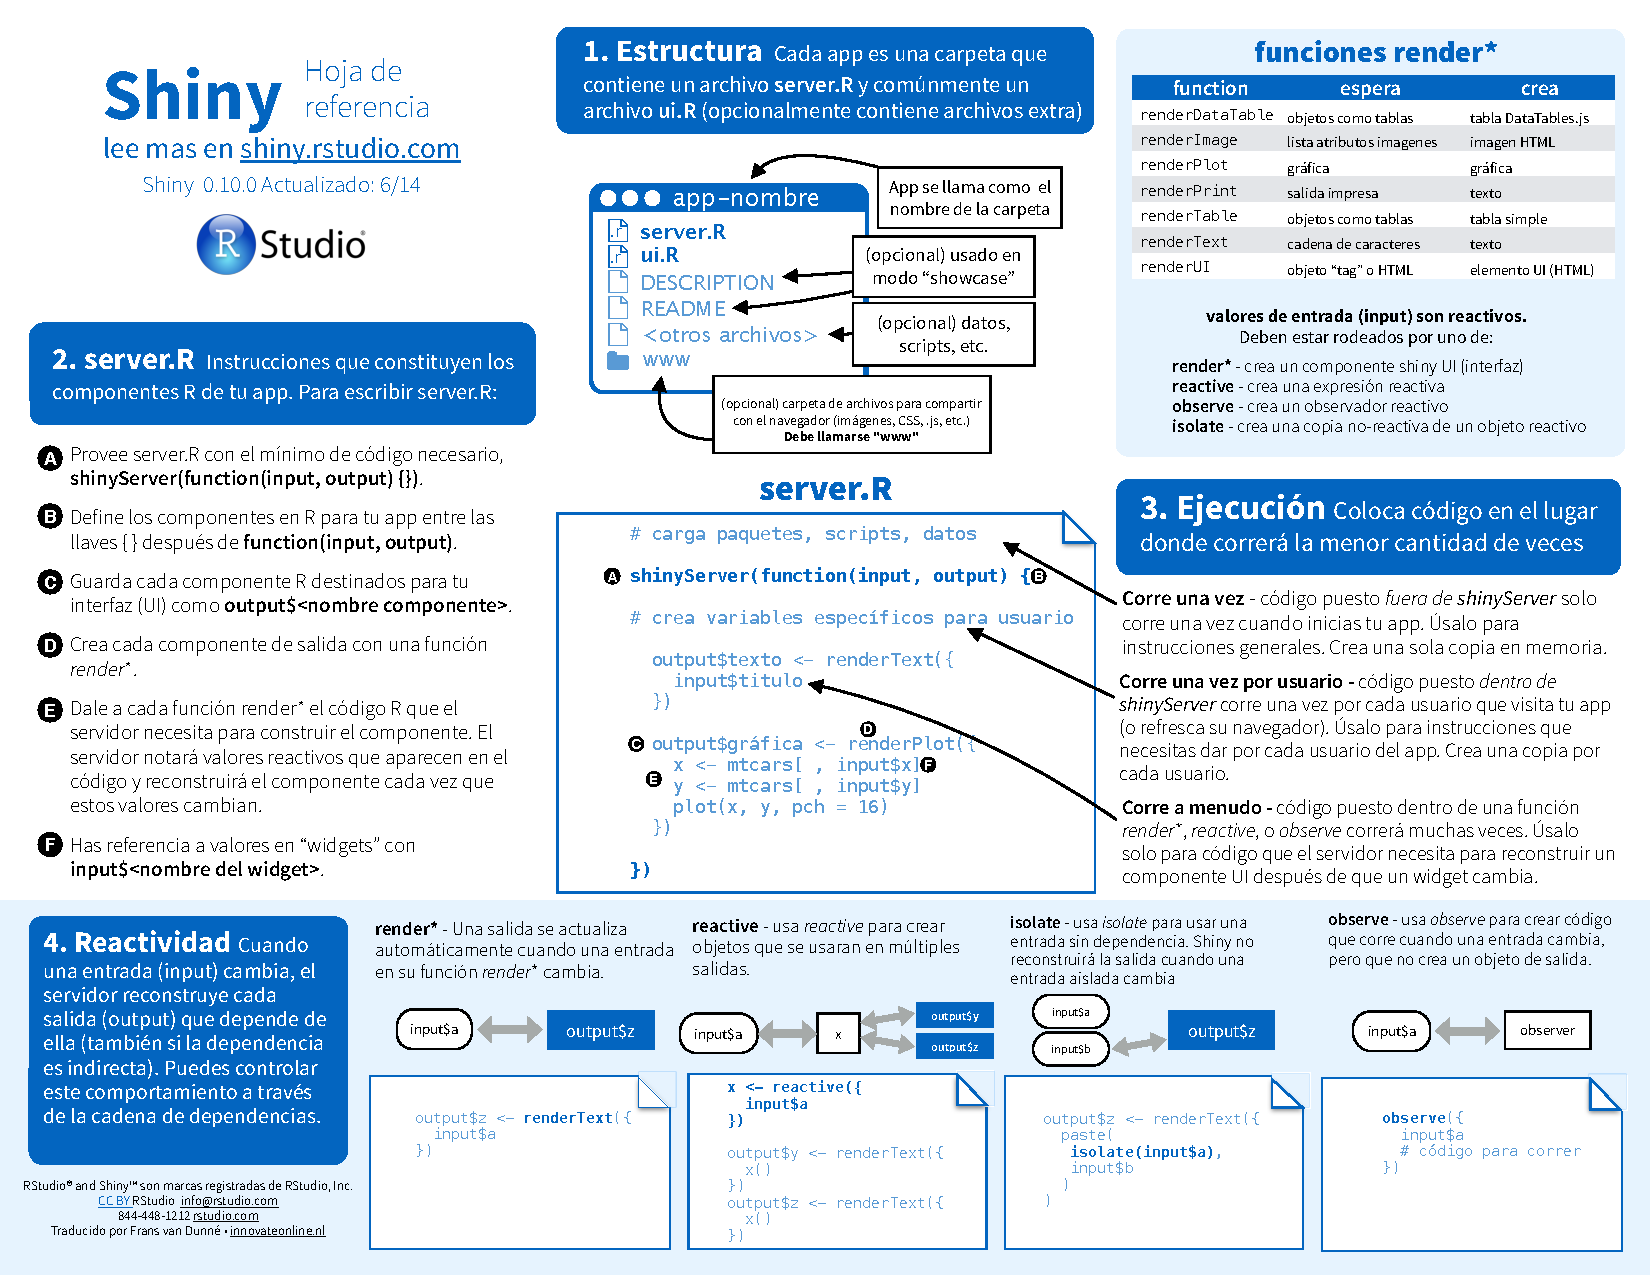
\includepdf[pages={1-2},scale=.78,pagecommand={},angle=90]{shiny-spanish.pdf}

%%%% Los cap'itulos inician con \chapter{T'itulo}, estos aparecen numerados y
%% se incluyen en el 'indice general.
%%
%% Recuerda que aqu'i ya puedes escribir acentos como: 'a, 'e, 'i, etc.
%% La letra n con tilde es: 'n.


%\setcounter{section}{1}
\chapter{Guías para usuario de Geneticae APP}


%%%% Los cap'itulos inician con \chapter{T'itulo}, estos aparecen numerados y
%% se incluyen en el 'indice general.
%%
%% Recuerda que aqu'i ya puedes escribir acentos como: 'a, 'e, 'i, etc.
%% La letra n con tilde es: 'n.


%\setcounter{section}{1}
\chapter{Código R de Geneticae APP}



%% Incluir la bibliograf'ia. Mirar el archivo "biblio.bib" para m'as detales
%% y un ejemplo.

\bibliography{biblio}

\end{document}
